\documentclass{emulateapj}
\submitted{{\it Submitted for publication in ApJL}}
\usepackage{multirow,color,wrapfig,ulem}
\usepackage {graphicx}

\usepackage{graphics}
\usepackage[dvips]{epsfig}

\newcommand{\manuscript}{paper }
\newcommand{\lcdm}{$\Lambda$CDM }
\newcommand{\mpc}{\rm{Mpc}}
\newcommand{\avg}[1]{\langle{#1}\rangle}  
\newcommand{\nscatt}{\langle N_{\rm  scatt}\rangle}
\newcommand{\ly}{{\ifmmode{{\rm Ly}\alpha~}\else{Ly$\alpha$~}\fi}}
\newcommand{\hMpc}{{\ifmmode{h^{-1}{\rm Mpc}}\else{$h^{-1}$Mpc }\fi}}   
\newcommand{\hGpc}{{\ifmmode{h^{-1}{\rm Gpc}}\else{$h^{-1}$Gpc }\fi}}   
\newcommand{\hmpc}{{\ifmmode{h^{-1}{\rm Mpc}}\else{$h^{-1}$Mpc }\fi}}  
\newcommand{\hkpc}{{\ifmmode{h^{-1}{\rm kpc}}\else{$h^{-1}$kpc }\fi}}  
\newcommand{\hMsun}{{\ifmmode{h^{-1}{\rm
        {M_{\odot}}}}\else{$h^{-1}{\rm{M_{\odot}}}$}\fi}}   
\newcommand{\hmsun}{{\ifmmode{h^{-1}{\rm
        {M_{\odot}}}}\else{$h^{-1}{\rm{M_{\odot}}}$}\fi}}   
\newcommand{\Msun}{{\ifmmode{{\rm {M_{\odot}}}}\else{${\rm{M_{\odot}}}$}\fi}}  
\newcommand{\msun}{{\ifmmode{{\rm {M_{\odot}}}}\else{${\rm{M_{\odot}}}$}\fi}}  
\newcommand{\lya}{{Lyman$\alpha$~}}
\newcommand{\clara}{{\texttt{CLARA}}~}
\newcommand{\rand}{{\ifmmode{{\mathcal{R}}}\else{${\mathcal{R}}$ }\fi}}  
\newcommand{\hs}{{\hspace{1mm}}}  
\newcommand{\kms}{{\ifmmode{{\mathrm{\,km\ s}^{-1}}}\else{\,km~s$^{-1}$}\fi}}

% definition to produce a "less than or similar to" symbol
\def\lsim{~\rlap{$<$}{\lower 1.0ex\hbox{$\sim$}}}

% definition to produce a "greater than or similar to" symbol
\def\gsim{~\rlap{$>$}{\lower 1.0ex\hbox{$\sim$}}}


\shorttitle{The Local Group in the Cosmic Web}
\shortauthors{Forero-Romero \& Gonz\'alez}

\begin{document}

\title{The Place of the Local Group in the Cosmic Web}
\author{J. E. Forero-Romero$^1$ and R. Gonz\'alez$^2$}
\affil{$^1$ Departamento de F\'{i}sica, Universidad de los Andes,
  Cra. 1 No. 18A-10, Edificio Ip, Bogot\'a, Colombia\\
  $^2$ Instituto de Astrof\'{i}sica, Pontificia Universidad Cat\'olica,
  Av. Vicu\~na Mackenna 4860, Santiago, Chile\\  
}
\email{je.forero@uniandes.edu.co}


\begin{abstract}
We explore the characteristics of the Local Group (LG)
location in the cosmic web using a cosmological simulation in the
$\Lambda$CDM cosmology.  We use the Hessian of the gravitational
potential to define the cosmic web, where regions are classified as
either peak, sheet, filament or void.  The LG in the simulations are
split into two samples.  The first is a general sample composed by
halo pairs with similar masses and isolation criteria as observed in
the LG.  The second is a subset with additional kinematic constaints.
We find that the pairs in the LG sample with all constraints are: i)
Preferentially located in filaments and sheets, ii) located in in a
narrow range of local overdensity $0<\delta<4$, web ellipticity
$0.1<e<1.0$ and prolateness $-0.5<p<0.5$.  iii) Clearly aligned with
the cosmic web, in particular for pairs in filaments/sheets the
orbital angular momentum tends to be perpendicular to the filament
direction or the sheet plane. A stronger alignment is present for the
vector linking the two halos, which lies along the filament or the
sheet plane.  We show that the first and second results are expected
trends with the LG total mass.  However, the strong alignment with the
cosmic web cannot be explained in the same way.


\end{abstract}

\begin{keywords}
{galaxies: Local Group --- dark matter}
\end{keywords}


\section{Introduction}
\label{sec:intro}

%lg rare
The spatial and kinematic configuration of the Local Group
(LG) galaxies is rare to find in the local Universe and in cosmological
simulations. 
The LG is dominated by the two big spirals MW and M31, the next
most-luminous galaxy is M33 which is $\sim 10$ times less massive than
M31, followed by several less luminous dwarf galaxies, up to a
distance of $\sim 3$\mpc.   
The velocity vector of M31, with a low
tangential velocity is consistent to a head-on collision orbit toward
the MW
\citep{2008MNRAS.386..461C,2012ApJ...753....8V,2012ApJ...753....7S}.   

Another feature of the Local group is the relatively low velocity
dispersion of nearby galaxies up to $\sim 8$ Mpc \citep[][and
  references therein]{1975ApJ...196..313S,2011MNRAS.415L..16A}. 
Environment around the Local Group has density quite close to the
average density of the universe
\citep{2003ApJ...596...19K,2005AJ....129..178K}. 
In addition, the
closest massive galaxy cluster, the Virgo Cluster, is $\approx
16.5\ \mpc$ away \citep{2007ApJ...655..144M}.  

All this combination of features make LG analogues rare to
find. 
Using numerical simulatons \citet{lganalogues} found less than
$2\%$ MW-sized halos reside in a pair similar to MW-M31 and in a
similar environment. 
Furthermore, if we select pairs constrained
within $2\sigma$ error fron current observational measurements of the
velocity components and distance to M31, there are only $46$ systems
in a cubic volume of $250$ \hmpc side, giving a number density $\sim
1.0\times 10^{-6}$Mpc$^{3}$, comparable to the abundance of massive
clusters.

\citet{2013ApJ...767L...5F} also studied MW-M31 pairs in numerical
simulations finding the typical quantities characterizing the orbital
parameters of the LG are rare among typical pairs, but not enough to
challenge the \lcdm model. 

Another definition of LG analogues is made by
\citet{2008MNRAS.384.1459L}, but despite differences ocurr in the
definitions and resulting fraction of LG analogues, all are in
agreement with a low frequency of these pairs. 
%lw08 also look lg analogues

%larger scales & lg env
To better understand the properties of the LG and how this uncommon
pair configuration fit in the cosmological context, an immediate
question arise. What else can we say of the LG at larger scales?. In
particular, which are the typical/prefered locations of these systems
within the Cosmic Web?. To what extent is this an expected
configuration in $\Lambda$CDM.

Looking the LG at larger scales we have it is located in a difuse and
warped filament/wall conecting Virgo Cluster with Fornax Cluster, some
nearby galaxies and groups members of this large structure are the
Maffei group, NGC $6744$, NGC $5128$, M$101$, M$81$, NGC$1023$, Cen A
group. At this scale, there is no evident alignment of the MW-M31
orbital plane with the local filament or the Virgo-Fornax
direction. However, if we look in a smaller volume below scales of
$\sim 6$ \mpc, there is a clear alignment of th the MW-M31 orbit with
a local plane as shown by Figure $3$ in \citet{2013AJ....146...69C}.  


%this paper.
In this \manuscript we study the large scale environment of LG 
analogues in the context of $\Lambda$CDM. We use the Bolshoi
simulation to explore in what structures they reside and if there is
any correlation or alignment with the cosmic web. The large scale
Environment is defined by the cosmic web components identified by
\citet{Tweb}, and we use the LG analogues computed by
\citet{lganalogues}. We pay spetial attention to quantify the kind of
environment that hosts LG pairs and their alignments with respect to
the prefered directions defined by the T-web. 
   
This \manuscript is organized as follows. In Section \ref{sec:simulation}
we present the N-body cosmological simulation and the algorithm to
define the cosmic web, next in \ref{sec:lg_analogues} we describe the
sample of LG analogues extracted from the simulation. In
Section \ref{sec:results} we presents our results to continue with a
discussion about their implications for our Local Group in Section
\ref{sec:discussion} to finally conclude in Section
\ref{sec:conclusions}. 


\section{Simulation and web finding algorithm}
\label{sec:simulation}

\subsection{The Bolshoi simulation}
We use the Bolshoi simulation of $\Lambda$CDM cosmology: $\Omega_{\rm
  m}=1-\Omega_{\Lambda}=0.27$, $H_0=70\,\rm km/s/Mpc$,
$\sigma_8=0.82$, $n_s=0.95$ \citep{2011ApJ...740..102K}, compatible
with the constraints from the WMAP satellite
\citep{hinshaw_etal13}. The simulation followed the evolution of dark
matter in a $250 \hmpc$ box with spatial resolution of $\approx
1h^{-1}$~kpc and mass resolution of $m_{\rm p}=1.35\times 10^8\ \rm
M_{\odot}$. Halos are identified with the BDM algorithm
\citep{1997astro.ph.12217K}. The BDM algorithm is  a spherical
overdensity halo finding algorithm and is designed to identify both
host halos and subhalos. 


\subsection{Cosmic web identification}
The web finding algorithm is based on the tidal tensor computed as the
Hessian of the  gravitational potential field

\begin{equation}
T_{ij} = \frac{\partial^2 \phi}{\partial r_i \partial r_j}, 
\end{equation}
%
where $r_{i}$, $i=1,2,3$ refers to the three spatial comoving
coordiates and $\phi$ is the gravitational potential renormalized to
follow the Poisson equation $\nabla^2\phi=\delta$ where
$\delta$ is the matter overdensity.  

This tensor is real and symmetric, which means that can be
diagonalized. 
We note its eigenvalues as $\lambda_1\geq \lambda_2\geq
\lambda_3$ and their corresponding eigenvectors $\hat{e}_1$,
$\hat{e}_2$ and $\hat{e}_3$. 
The web classification compares each one
of the three eigenvalues to a threshold value $\lambda_{\rm th}$. 
If
the three, two, one or zero eigenvalues are larger than this threshold
the region is classified as peak, filament, sheet or void,
respectively.  

\cite{Tweb} performed a detailed study for the topology of the
cosmic web and its visual counterpart as a function of the parameter
$\lambda_{\rm th}$. 
They found that reasonable results in terms of the
volume fraction occupied by voids, the visual inspection and the halo
populations in each web type can be reached by values of $0.2<\lambda_{\rm
th}<0.4$. 
In this \manuscript we choose the value of $\lambda_{\rm
  th}=0.3$ to proceed with our analysis. 
This is only relevant to the classification of the simulation into web
elements. Other results are completeley independent of this
choice. Nevertheless we have checked that the main conclusions of this
work do not depend on the choise of $\lambda_{\rm th}$.


The algorithm to compute the potential is grid based. 
First we interpolate the density into a cubic grid with a
Cloud-In-Cell (CIC) scheme and smooth it with a gaussian kernel. 
Then we obtain the gravitational potential using FFT methods and use finite differences
to compute the Hessian at every point in the grid. 
In our case we have used a grid size on and a gaussian smoothing with
two times larger as the typical separation between the two halos in the Local Group. 
The purpose of this choice is to have both halos in the pair a common
environment. 
In this \manuscript we use a grid spacing of $s=0.97$ \hMpc,
corresponding to a $256^3$ grid in the Bolshoi volume. 
The scale for the gaussian smoothing uses the same value.

We use the matter overdensity, ellipticity and the prolatenes to
further characterize the web. 
These quantities are defined in terms of the
eigenvalues as follows 
%
\begin{equation}
\delta = \lambda_1 + \lambda_2 + \lambda_3,
\end{equation}
%
\begin{equation}
e= \frac{\lambda_3 - \lambda_1}{2(\lambda_1 + \lambda_2 + \lambda_3)}, 
\end{equation}
%
\begin{equation}
p= \frac{\lambda_1 + \lambda_3 - 2\lambda_2}{2(\lambda_1 + \lambda_2 +
  \lambda_3)}.
\end{equation}

We also measure the alignment of the LG halos with respect to the
cosmic web defined by the eigenvector.
To this end we characterize each LG pair by two vectors. 
The first is $\hat{n}$, the vector marking the axis along the orbital angular
momentum of the pair, normal to its orbital plane; the second is
$\hat{r}$, the vector that connects the halos in the pair. 
We quantify the alignment using the absolute value of the cosinus of
the angle between the two vectors of interest $\mu=|\hat{e}_i \cdot
\hat{n}|$ or $\mu=|\hat{e}_i\cdot \hat{r}|$, where $i=1,2,3$. 


The data of the BDM halos and the Tweb is publicly available through
a database located at \url{http://www.cosmosim.org/}. A detailed
description of the database structure was presented by \cite{Riebe2013}.

\section{Local Group Analogues}
\label{sec:lg_analogues}

To construct a sample of the MW-M31 pairs at $z\approx 0$, we use a
series of simulation snapshots  at $z<0.1$ (since the last $\approx
1.3$ Gyr) spaced by $\approx 150-250$ Myr. 
This is done because a particular configuration of MW and M31 is transient and
corresponds to a relatively small number of systems at one
snapshot. 
By using multiple snapshots we can increase the sample of systems in
such configuration during a period of time in which secular
cosmological evolution is small.  

The LG analogues or General Sample (GS) in this paper are pairs selected in
relative isolation, and in a wide range of masses from  $M_{200c}=5
\times 10^{11}$ \msun $ $ to $ 5 \times 10^{13}$ \msun.  
Isolation criteria includes a pair closer than $1.3$\mpc, and with no
massive neighbors within $5$\mpc.
In addition we require that pairs have no Virgo-like neighbor halo
with mass $M_{200c}>1.5 \times 10^{14}\ \rm M_{\odot}$ within $12$
Mpc.  
We have $5480$ pairs under these general criteria. 
A full description of the selection criteria can be found in
\citet{lganalogues,sat}.   

We also define two subsamples more closely related to the MW-M31 
dynamics according to the tolerance in additional constraints.
A sample named $2\sigma$, correspondig to LG analogues constrained by
two times the observational errors in the orbital values (radial
velocity, tangential velocity, and separation), and a more relaxed
sample named $3\sigma$ for LG analogues constrained by three times
observational errors accordingly. 
The number of pairs in each sample is $46$ and $120$ respectively,
notice we have less pairs than in \citet{lganalogues} results, since
we removed pairs which are too close at $z=0$, i.e. their virial radii
overlaps, also we removed a couple pairs that merged or change their
mass more than $20\%$ at present time since they were detected at
$z<0.1$. 


\section{Results}
\label{sec:results}

\begin{table*}
\begin{center}
\begin{tabular}{ccccc}\hline\hline
Sample & Peak & Filament & Sheet & Void\\
       & $n$ (\%) & $n$ (\%) & $n$ (\%) & $n$ (\%) \\\hline
2$\sigma$ & 4 (8.7) & 24 (52.2) &  17 (36.7) & 1 (2.2)\\
3$\sigma$ & 10 (8.3) & 58 (48.3) & 47 (39.2) & 5 (4.2)\\  
General & 1312 (23.9) & 1472 (26.9) & 1769 (32.3) & 927 (16.9)\\
General ($12.1<\log_{10} M_{\rm LG}/\Msun<12.3$)& 8 (1.4) & 334 (55.5) & 259
(43.0) & 1 (0.1)\\
\hline\hline
\end{tabular}
\caption{
Number of pairs in the four different kinds of environments for each
of the three samples presented in Section \ref{sec:lg_analogues}. 
In parethesis the same number as a percentage of the total population.
The last line in the table corresponds to the general sample with an
additional mass cut for the total pair mass.  
\label{table:web_type}}
\end{center}
\end{table*}



\begin{figure}
\begin{center}
  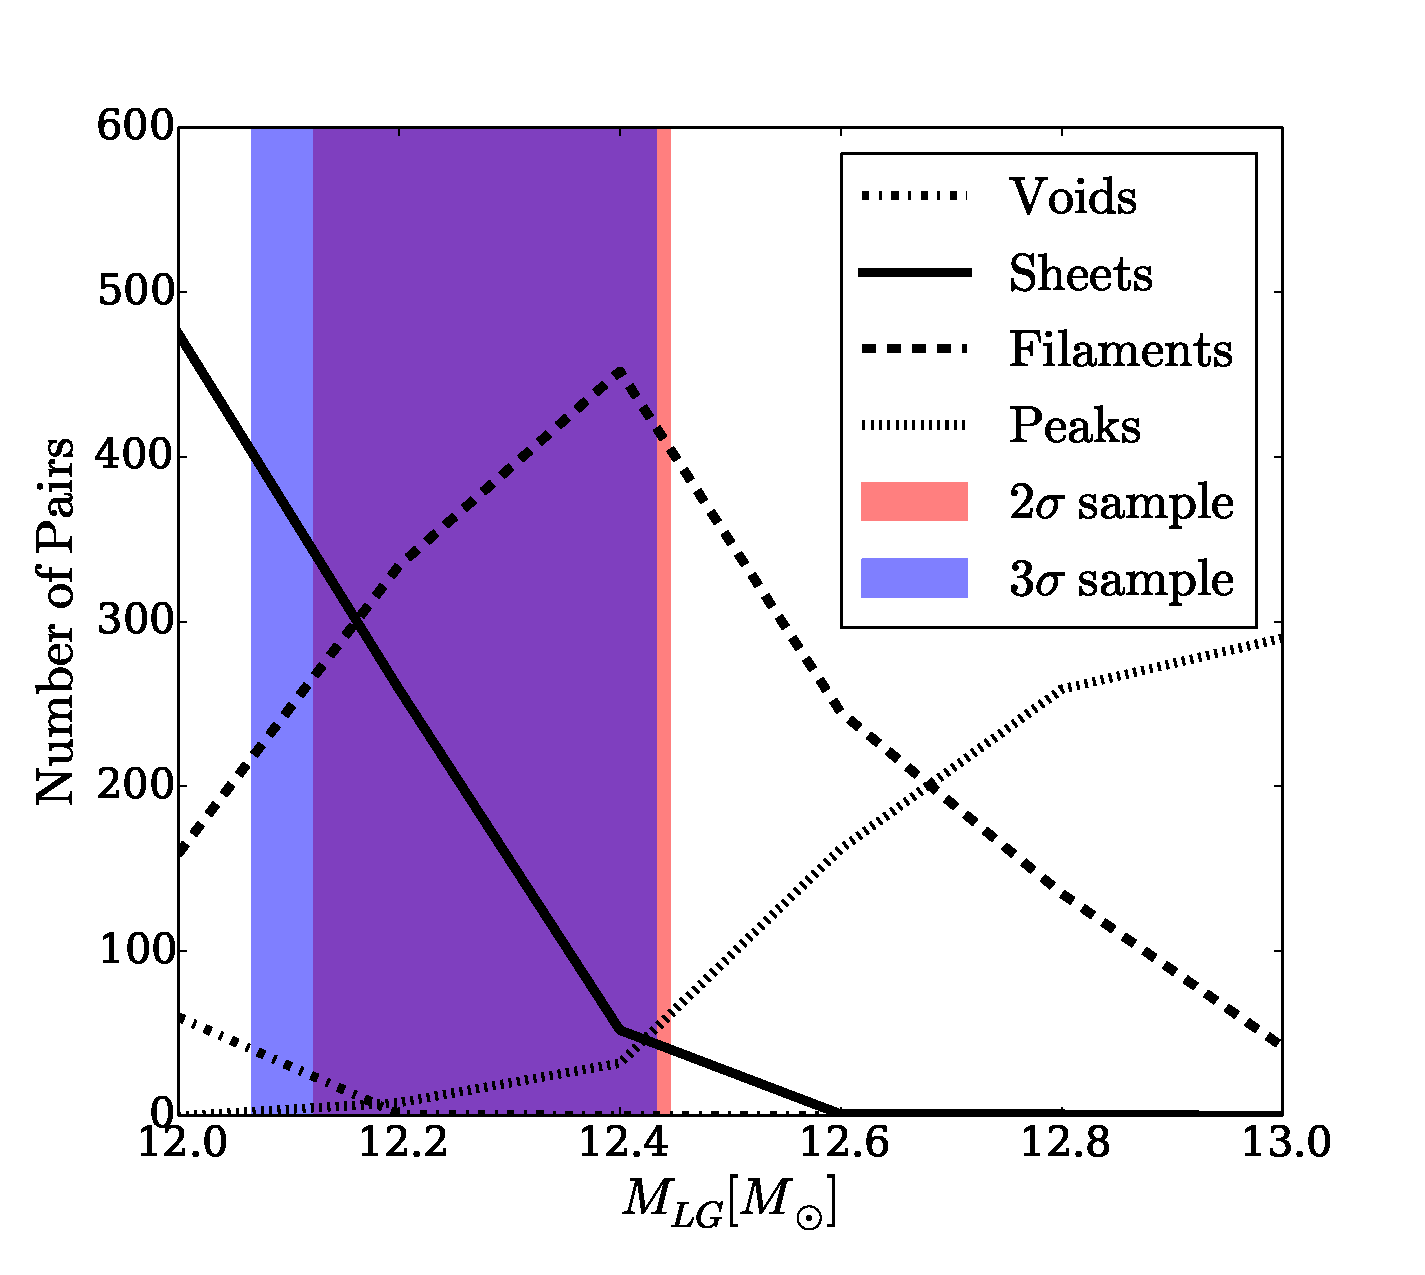
\includegraphics[width=0.48\textwidth]{histogram_mass_distro.pdf}
\caption{Mass distribution of pairs in the different environments
for the general sample.
The shaded regions show the mass ranges of $2\sigma$ and $3\sigma$
samples.  
\label{fig:median_fraction}}
\end{center}
\end{figure}


\begin{figure*}
\begin{center}
  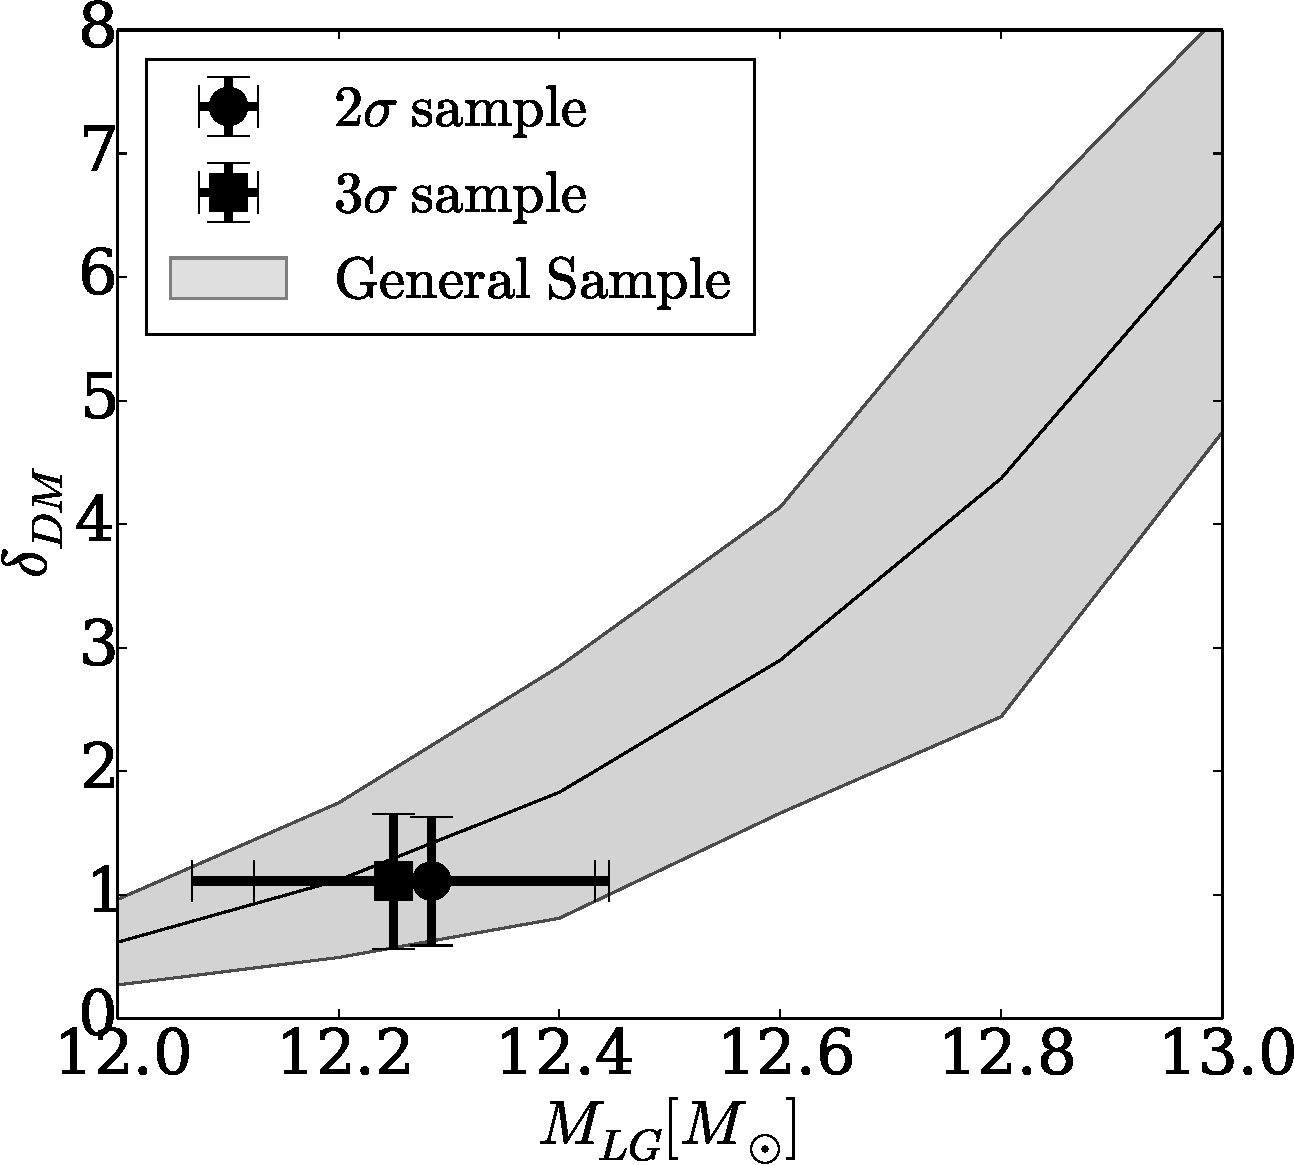
\includegraphics[width=0.31\textwidth]{median_mass_overdensity.pdf} 
  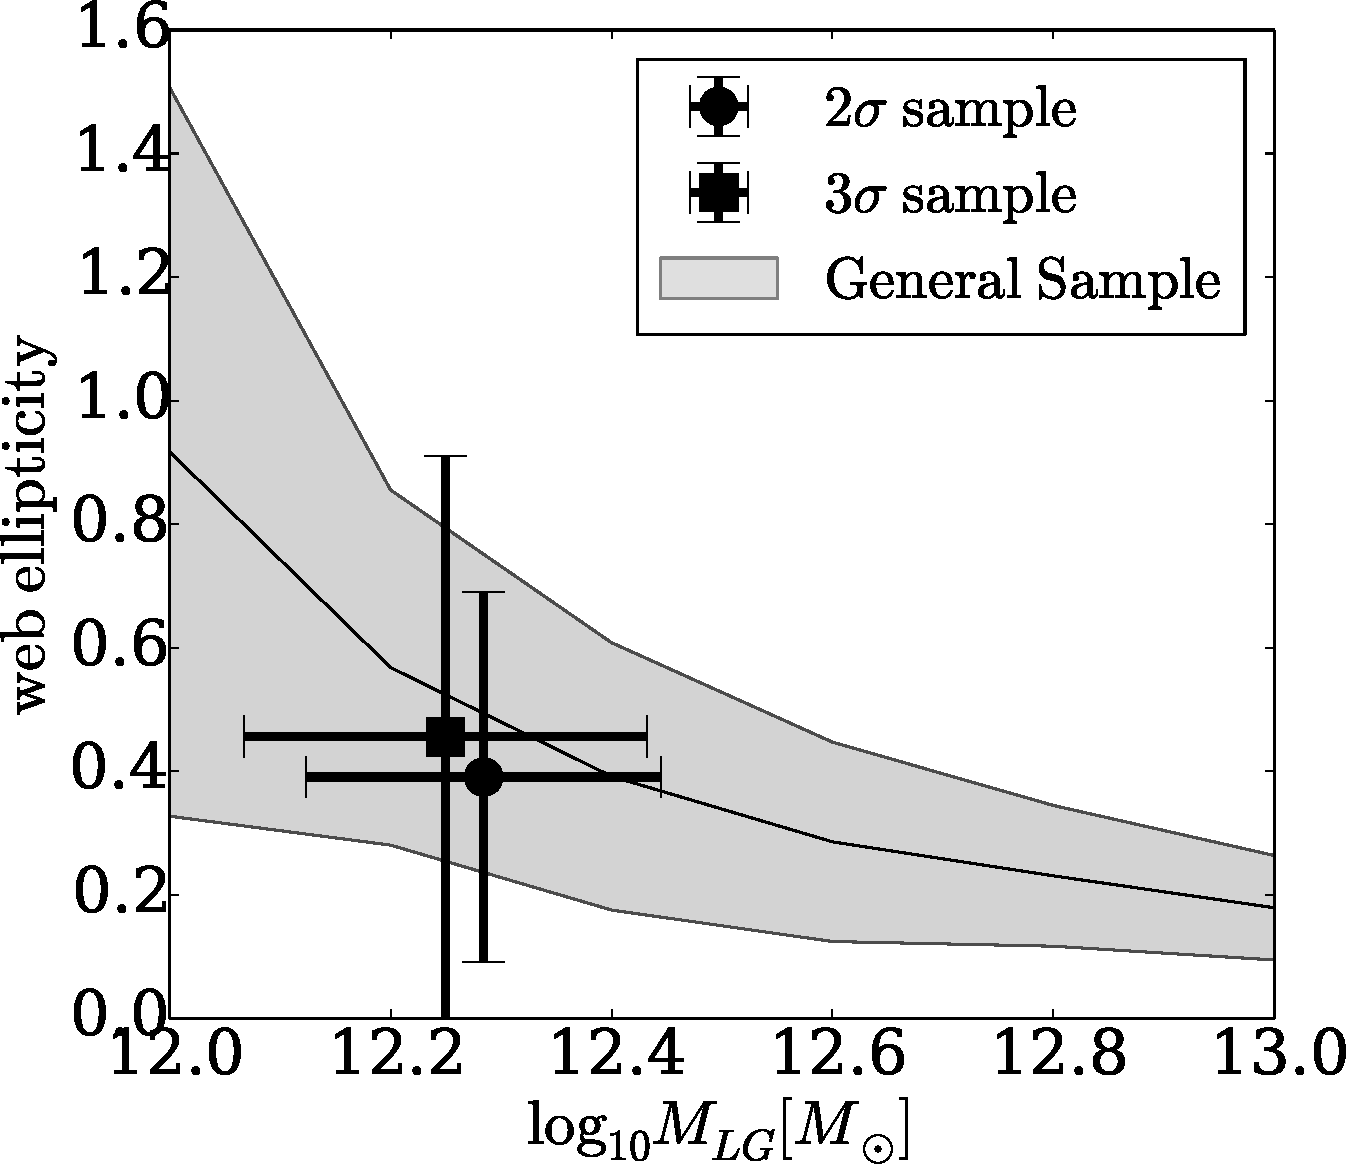
\includegraphics[width=0.32\textwidth]{median_mass_ellipticity.pdf} 
  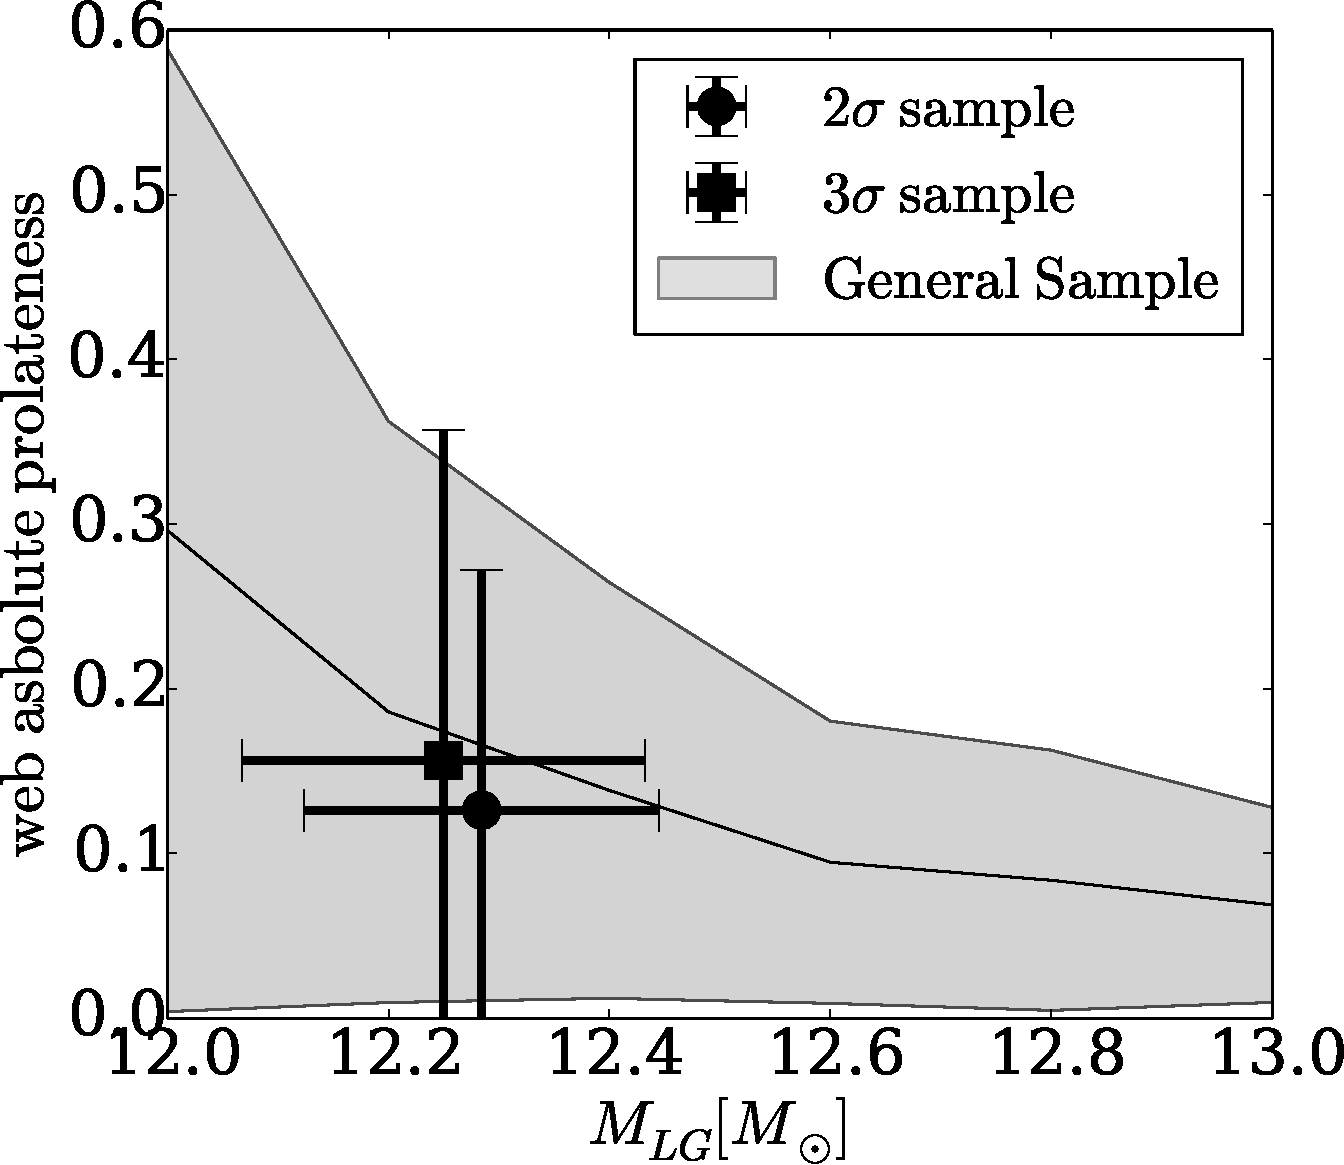
\includegraphics[width=0.32\textwidth]{median_mass_prolateness.pdf} 
\caption{Mass dependency of the average dark matter overdensity (left),
  web ellipticity (middle) and web absolute value prolateness (right) at the
  pair location.
\label{fig:median_overdensity}}
\end{center}
\end{figure*}




\begin{figure}
\begin{center}
  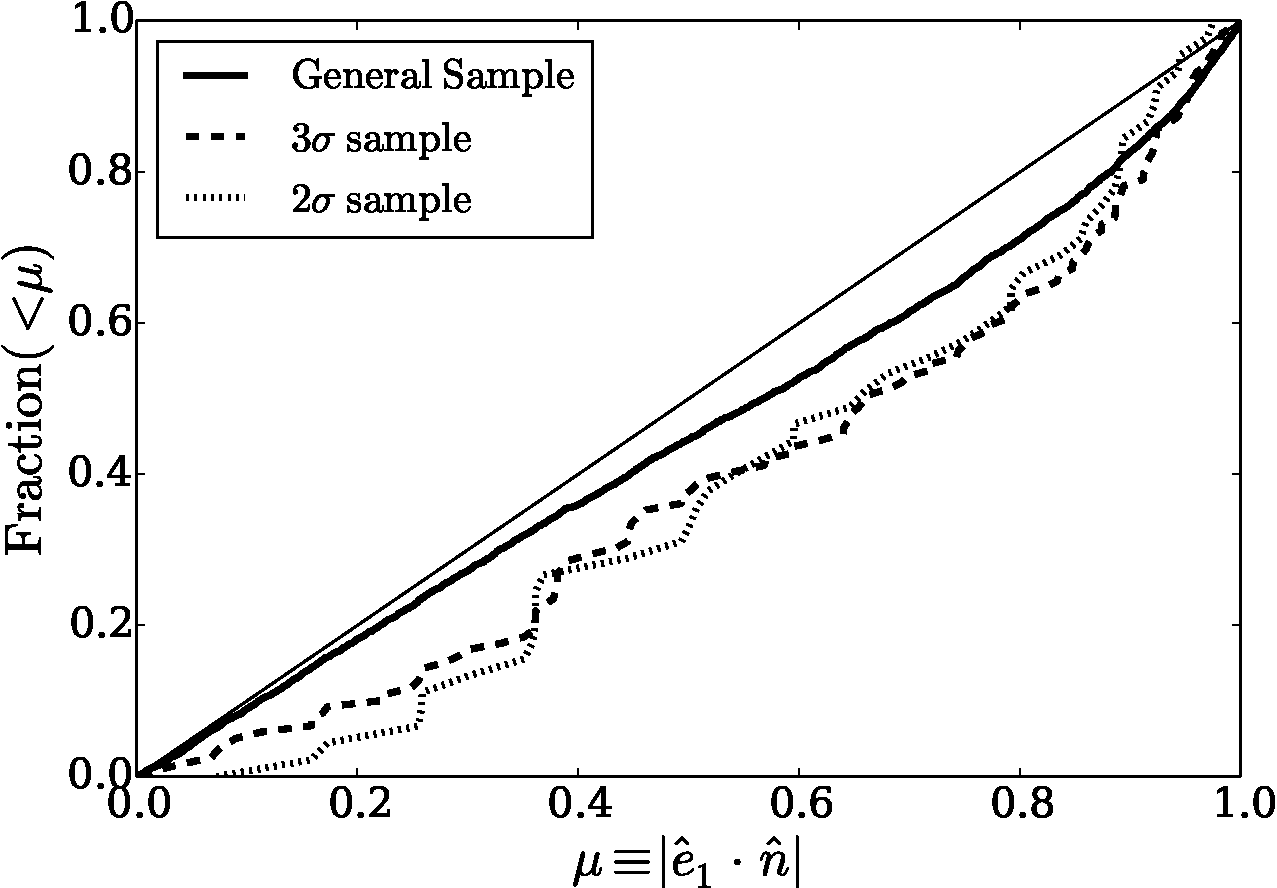
\includegraphics[width=0.48\textwidth]{alignments_e1_n_all_environments.pdf} 
  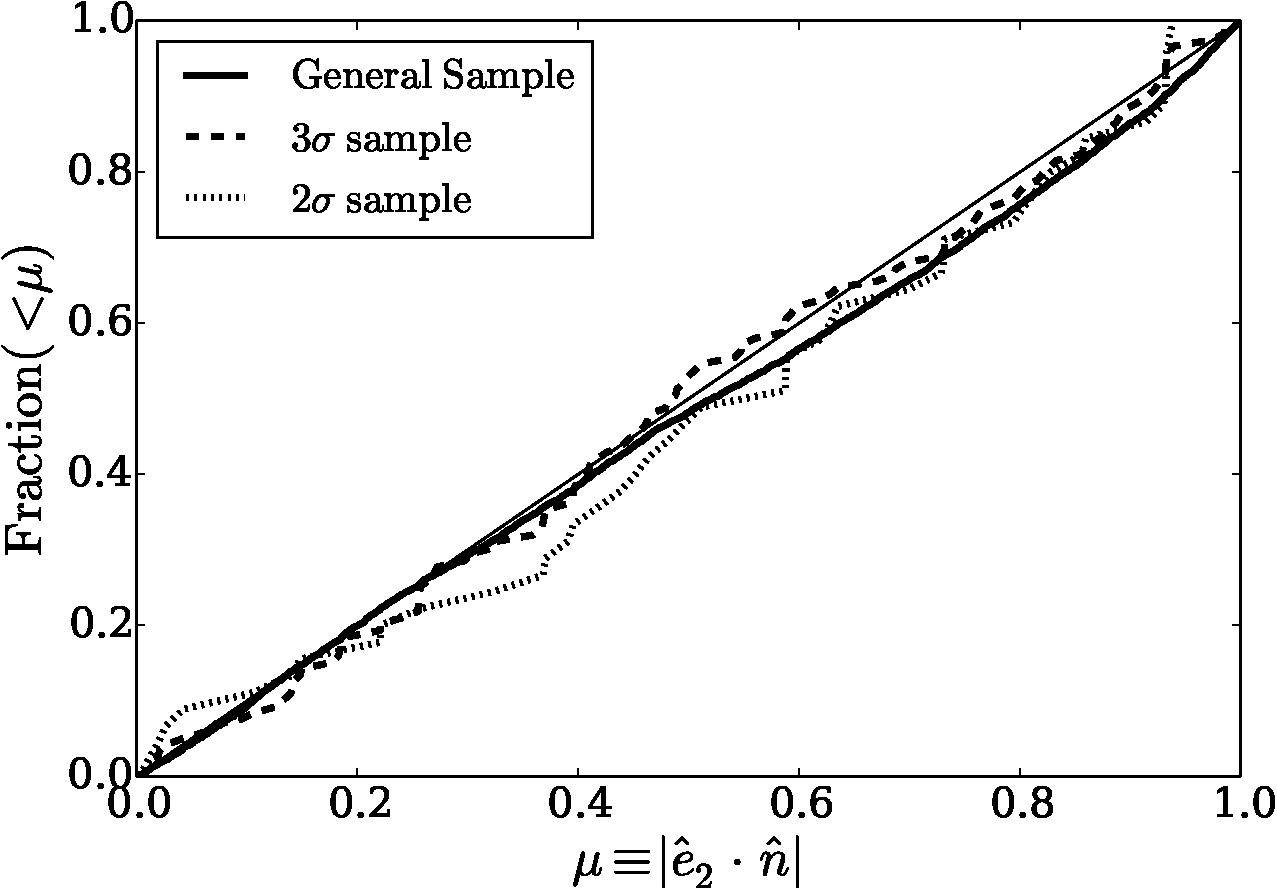
\includegraphics[width=0.48\textwidth]{alignments_e2_n_all_environments.pdf} 
  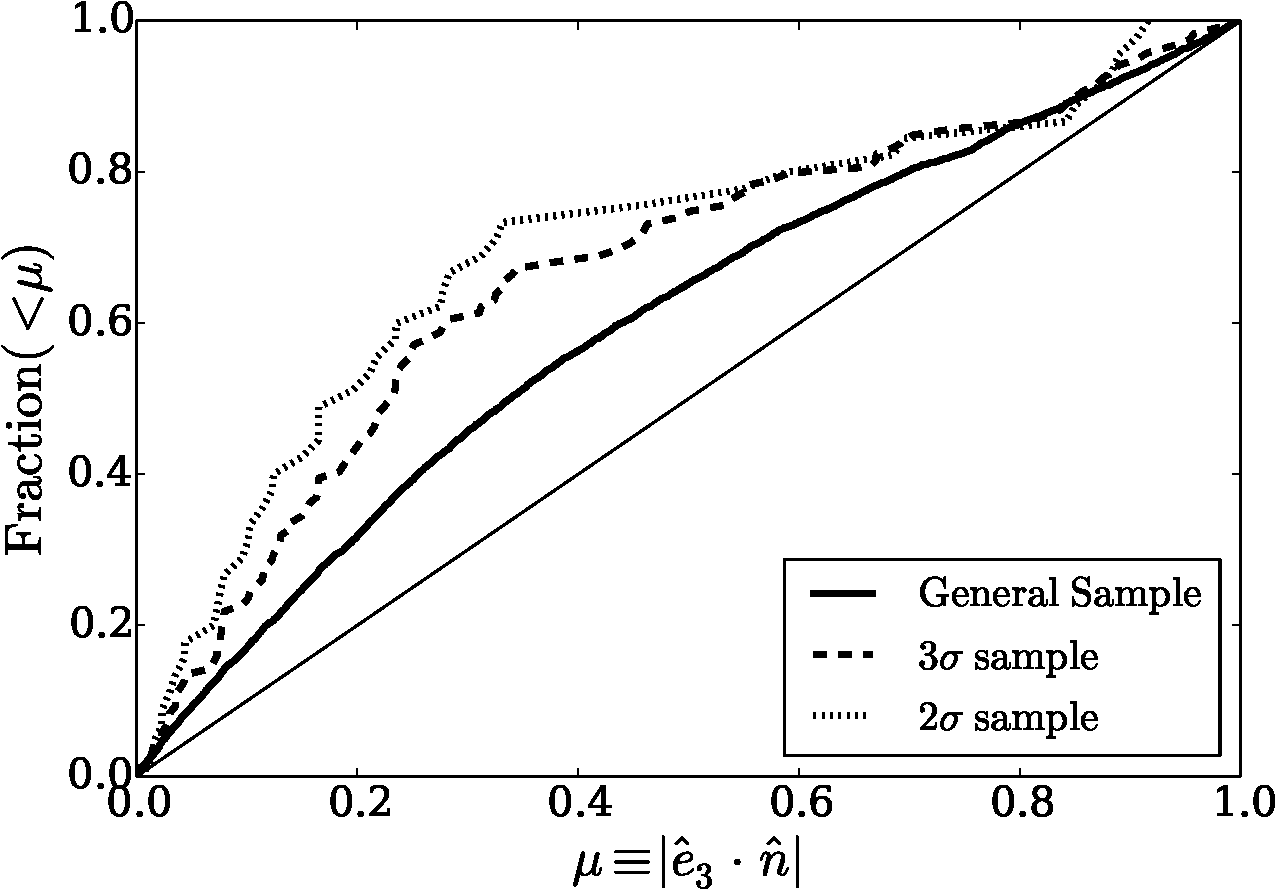
\includegraphics[width=0.48\textwidth]{alignments_e3_n_all_environments.pdf} 
\end{center}
\caption{Cumulative distributions for the alignment between the normal
  vector to the pair orbital plane, $\hat{n}$, and the three eigenvectors in
  the Tweb.
    \label{fig:alignment_n}}  
\end{figure}



\begin{figure}
\begin{center}
  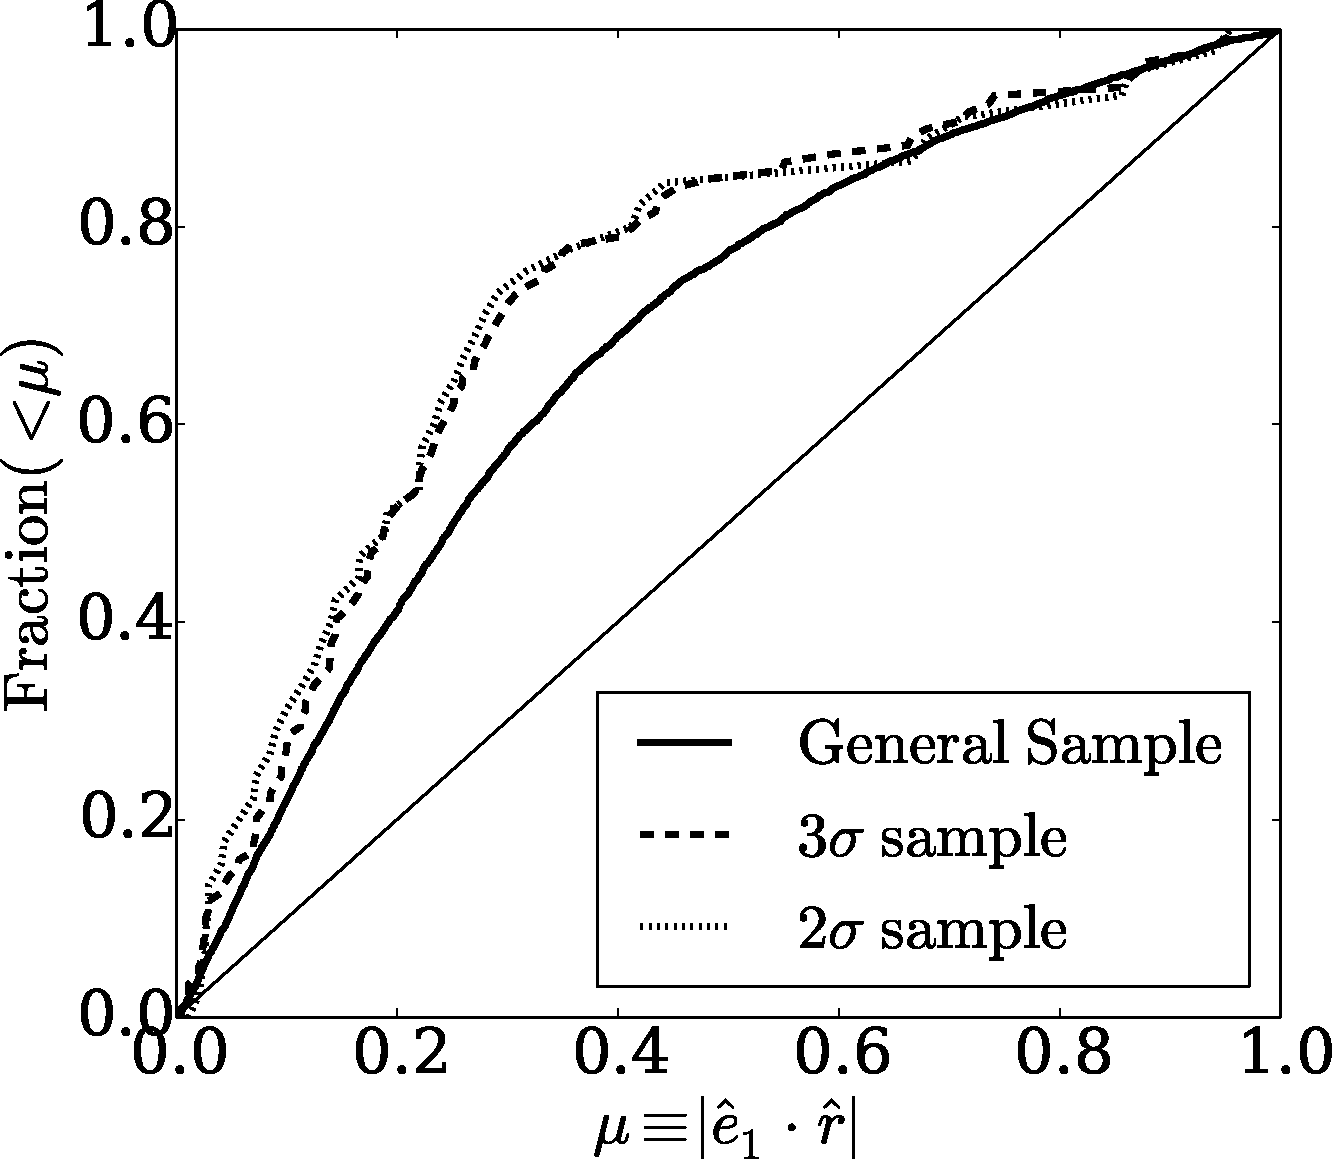
\includegraphics[width=0.48\textwidth]{alignments_e1_r_all_environments.pdf} 
  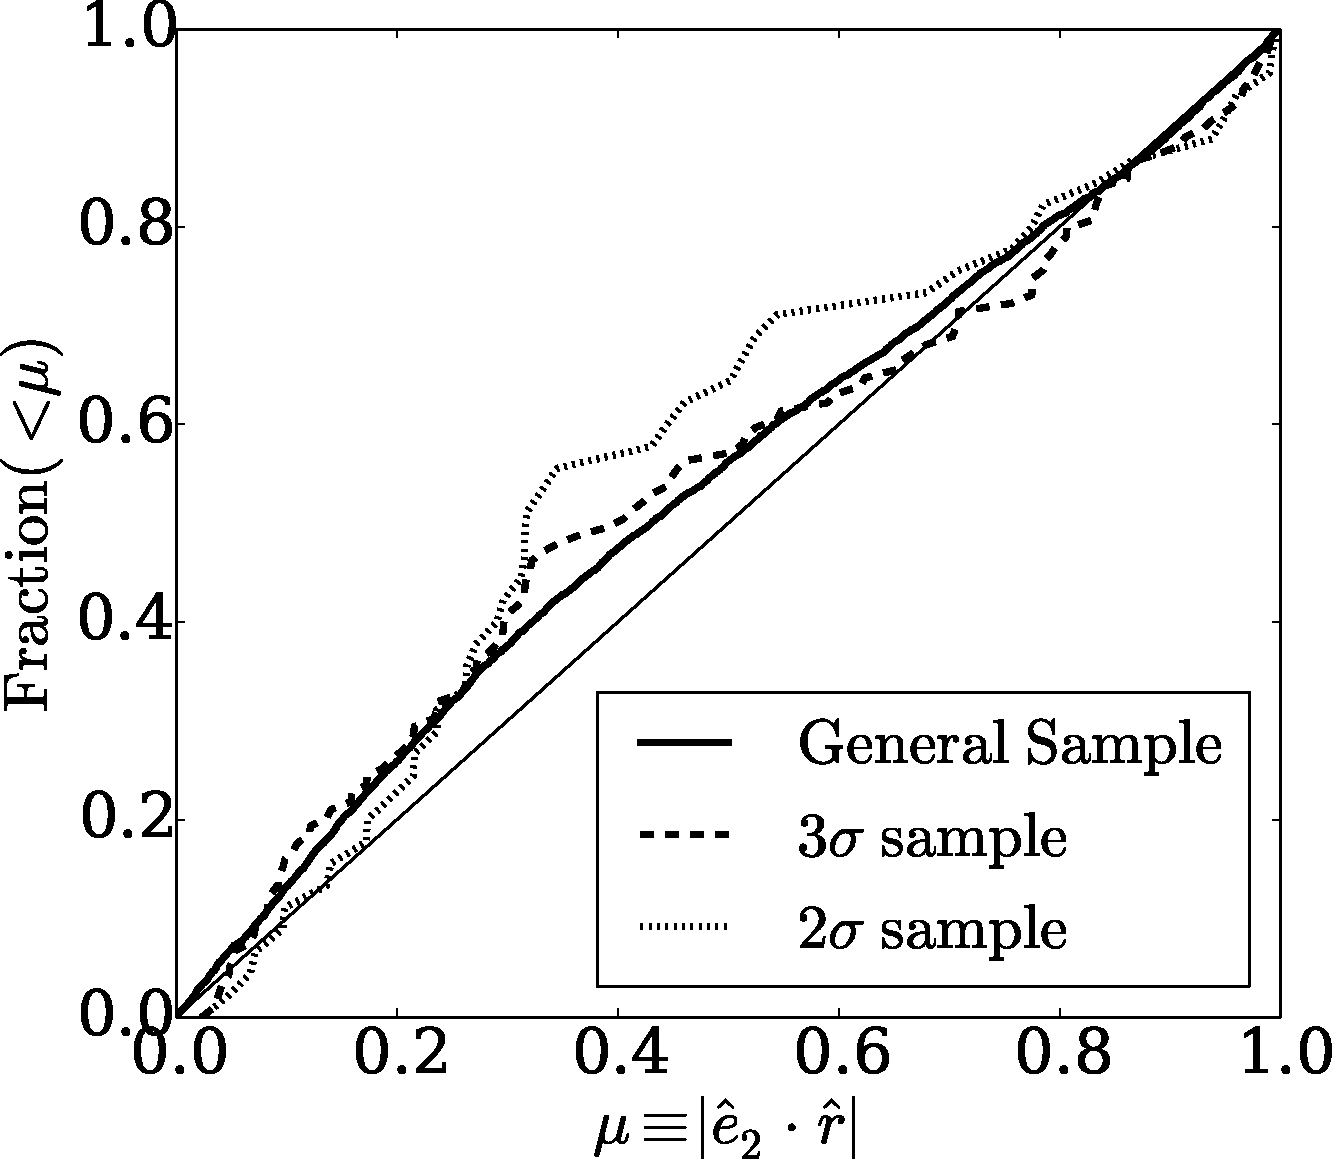
\includegraphics[width=0.48\textwidth]{alignments_e2_r_all_environments.pdf} 
  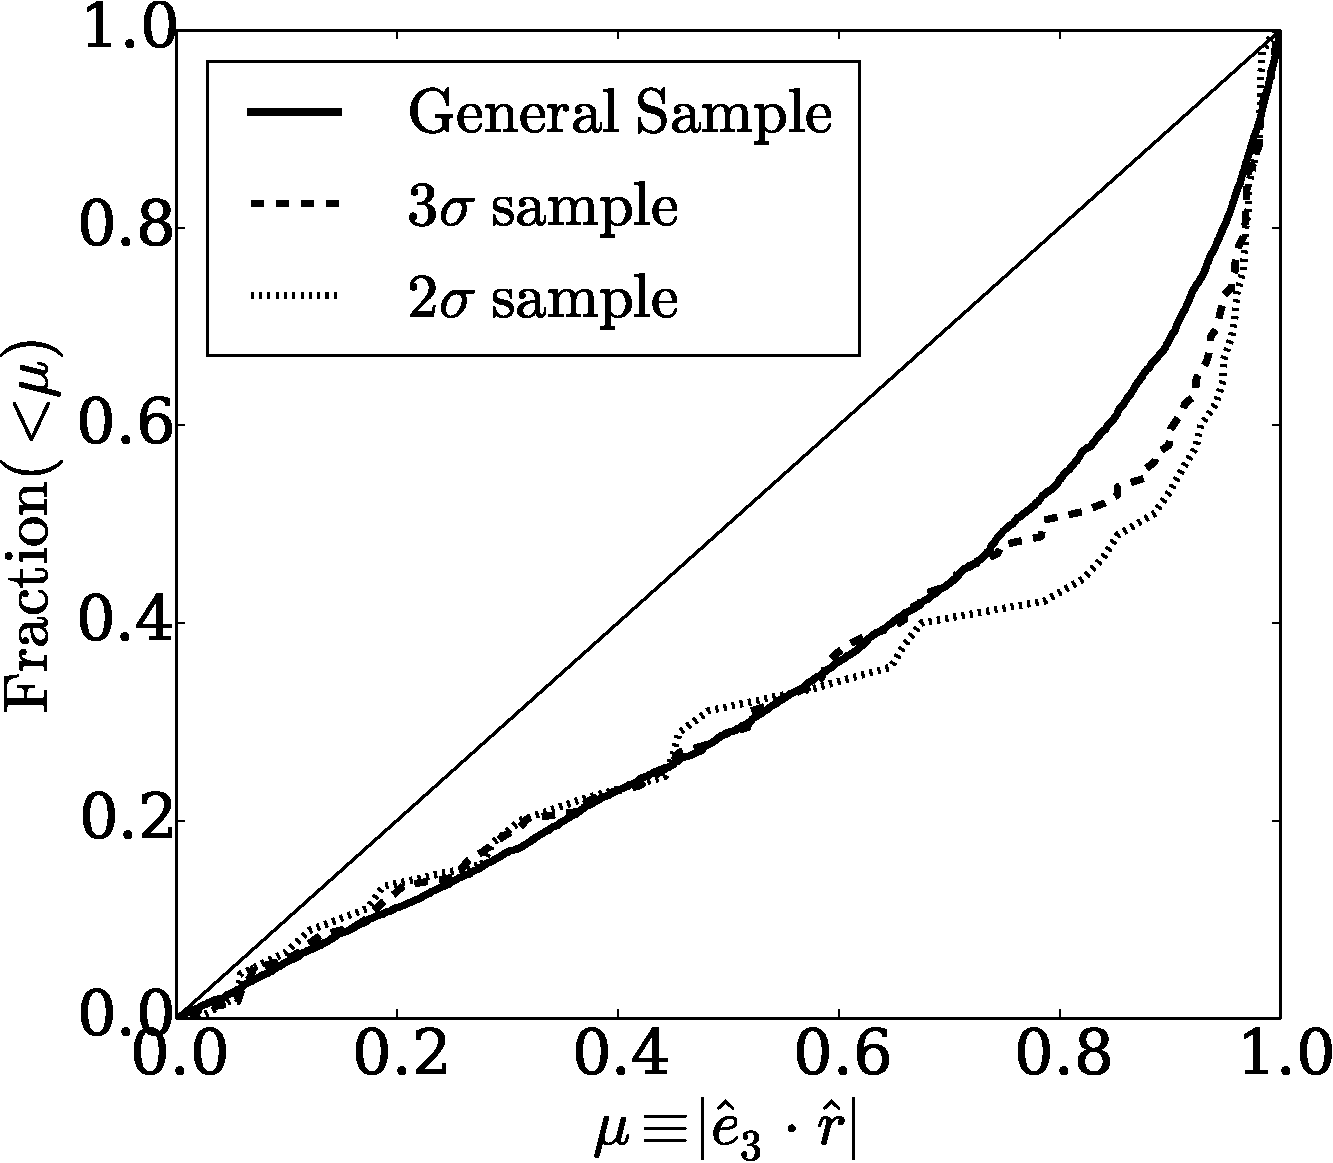
\includegraphics[width=0.48\textwidth]{alignments_e3_r_all_environments.pdf} 
\end{center}
\caption{Cumulative distributions for the alignment between the vector
  linking the two halos in the pair, $\hat{r}$, and the three
  eigenvectors in the Tweb.
    \label{fig:alignment_r}}  
\end{figure}


%\begin{figure}
%  \begin{center}
%    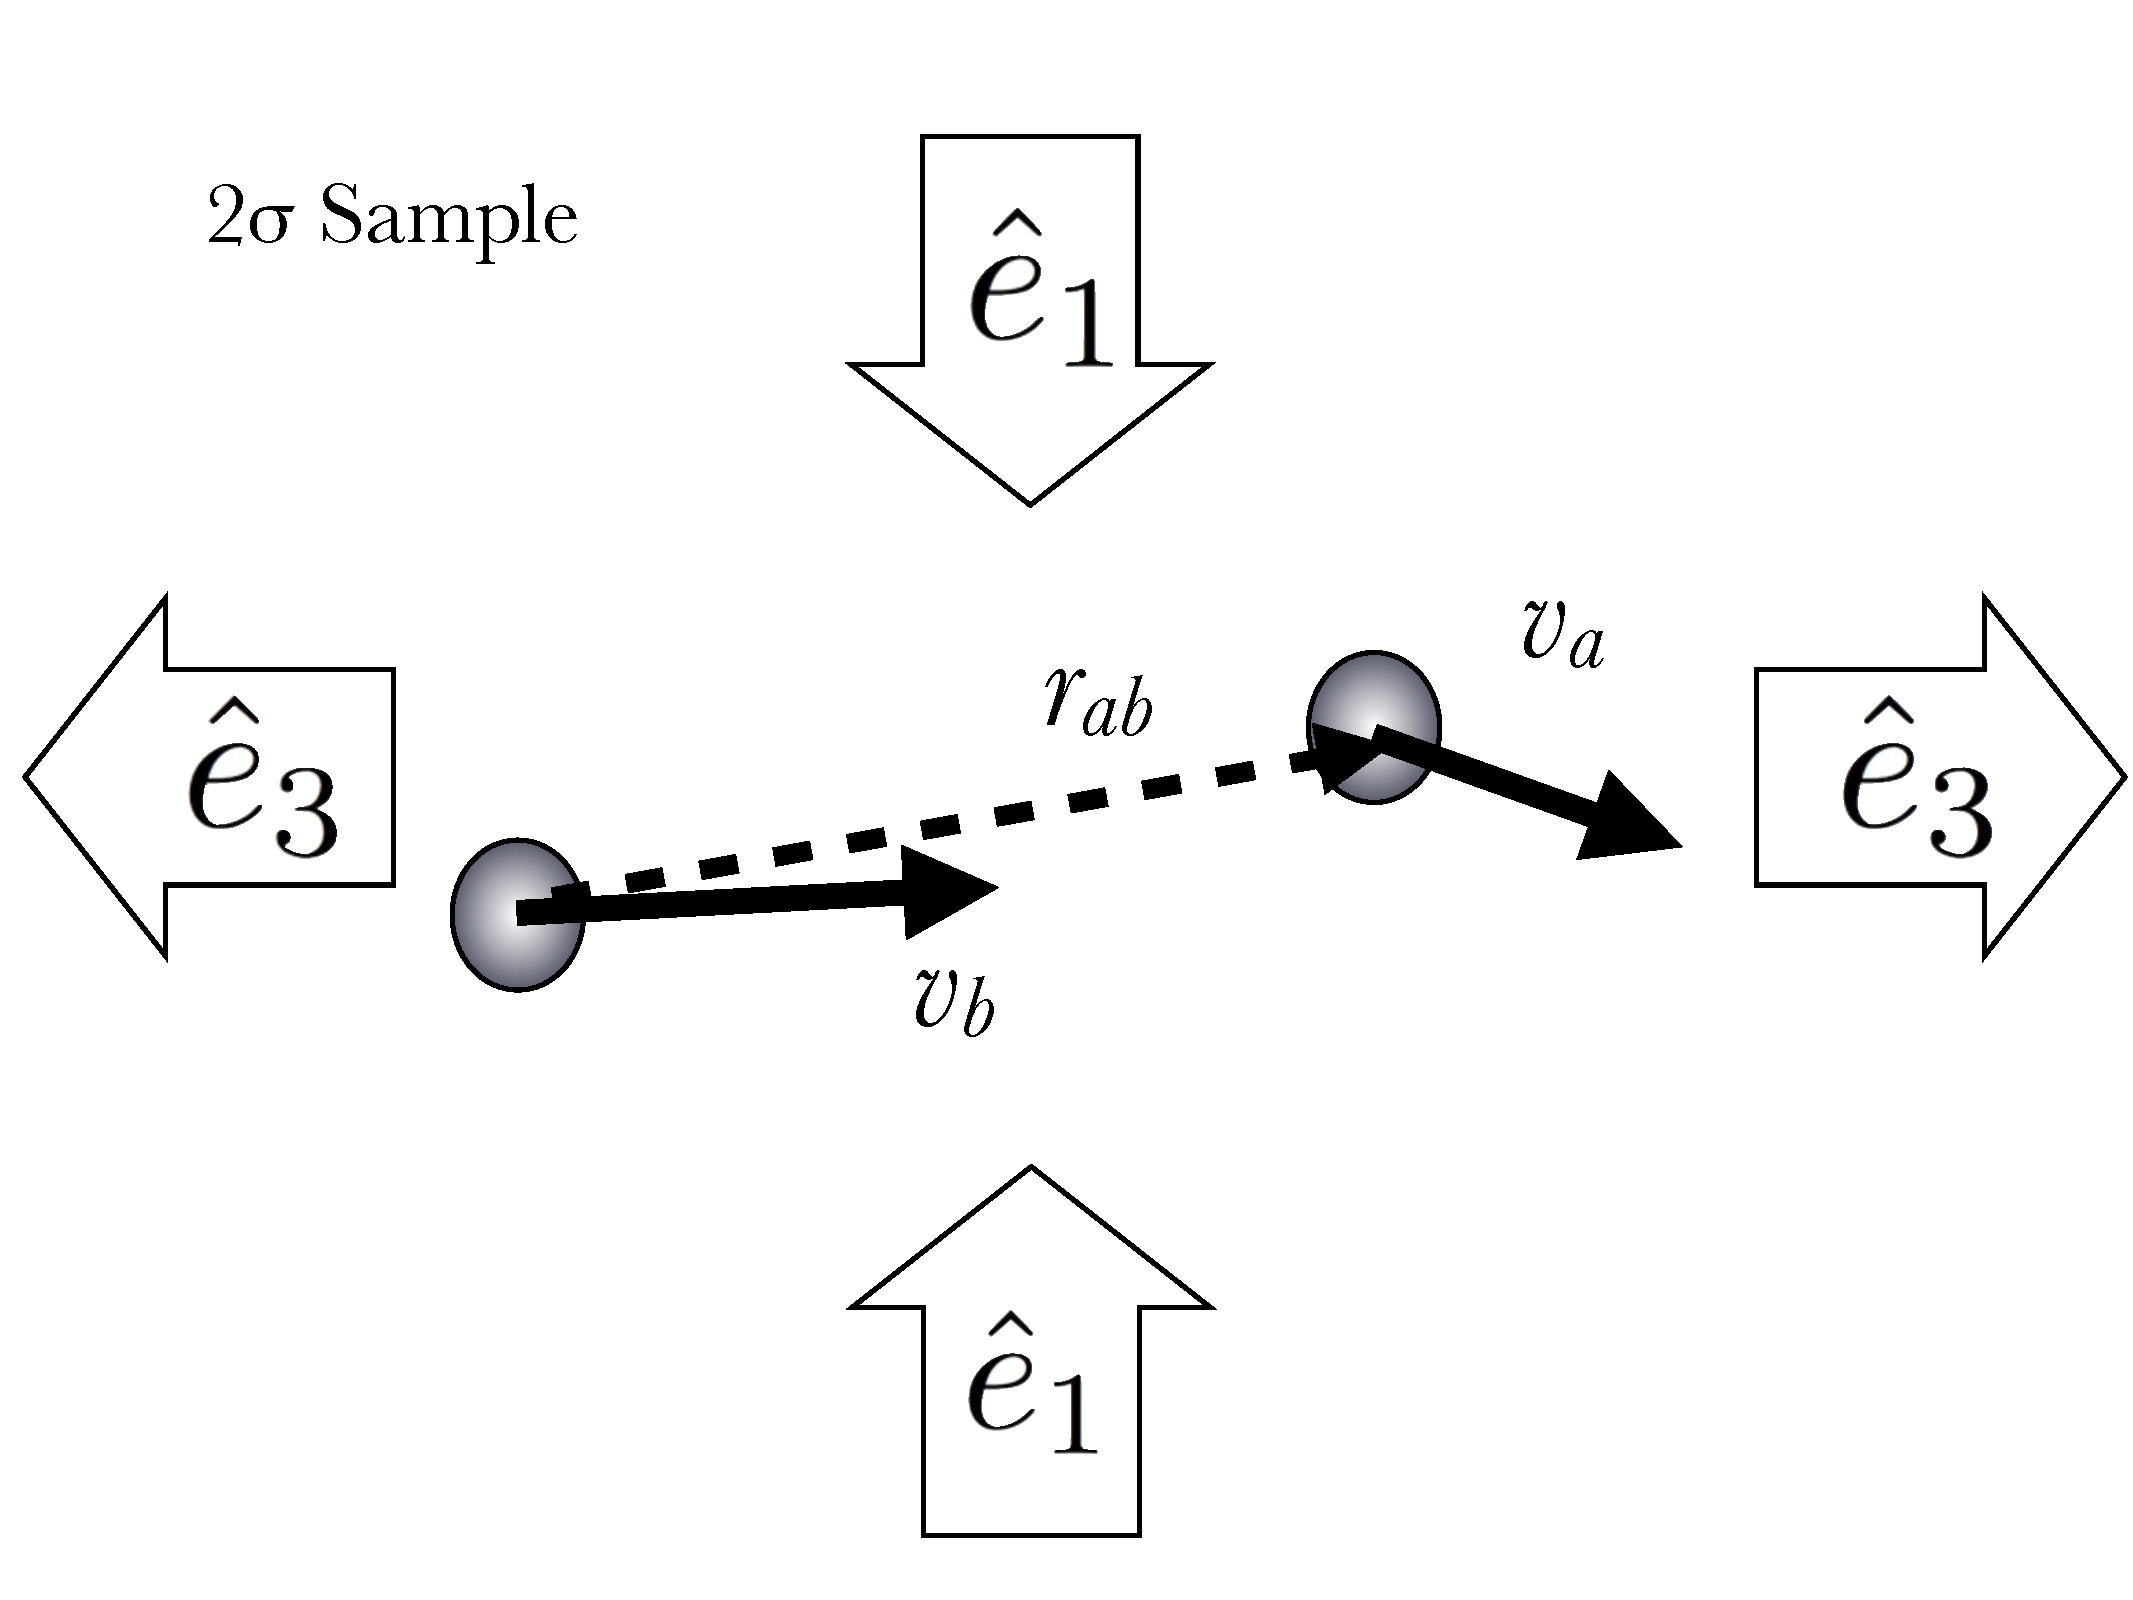
\includegraphics[width=0.48\textwidth]{scheme.pdf}
%    \caption{Schematic picture of the strongest alignment tendencies in
%      the the General and $2\sigma$-$3\sigma$ samples. The alignment
%      between the peculiar velocities and the $\hat{e}_3$ eigenvector was
%      reported in \citet{ForeroRomero2014} for all halos regardles of its
%      mass.
%      \label{fig:scheme}}
%  \end{center}
%\end{figure}



%\begin{figure}
%\begin{center}
%  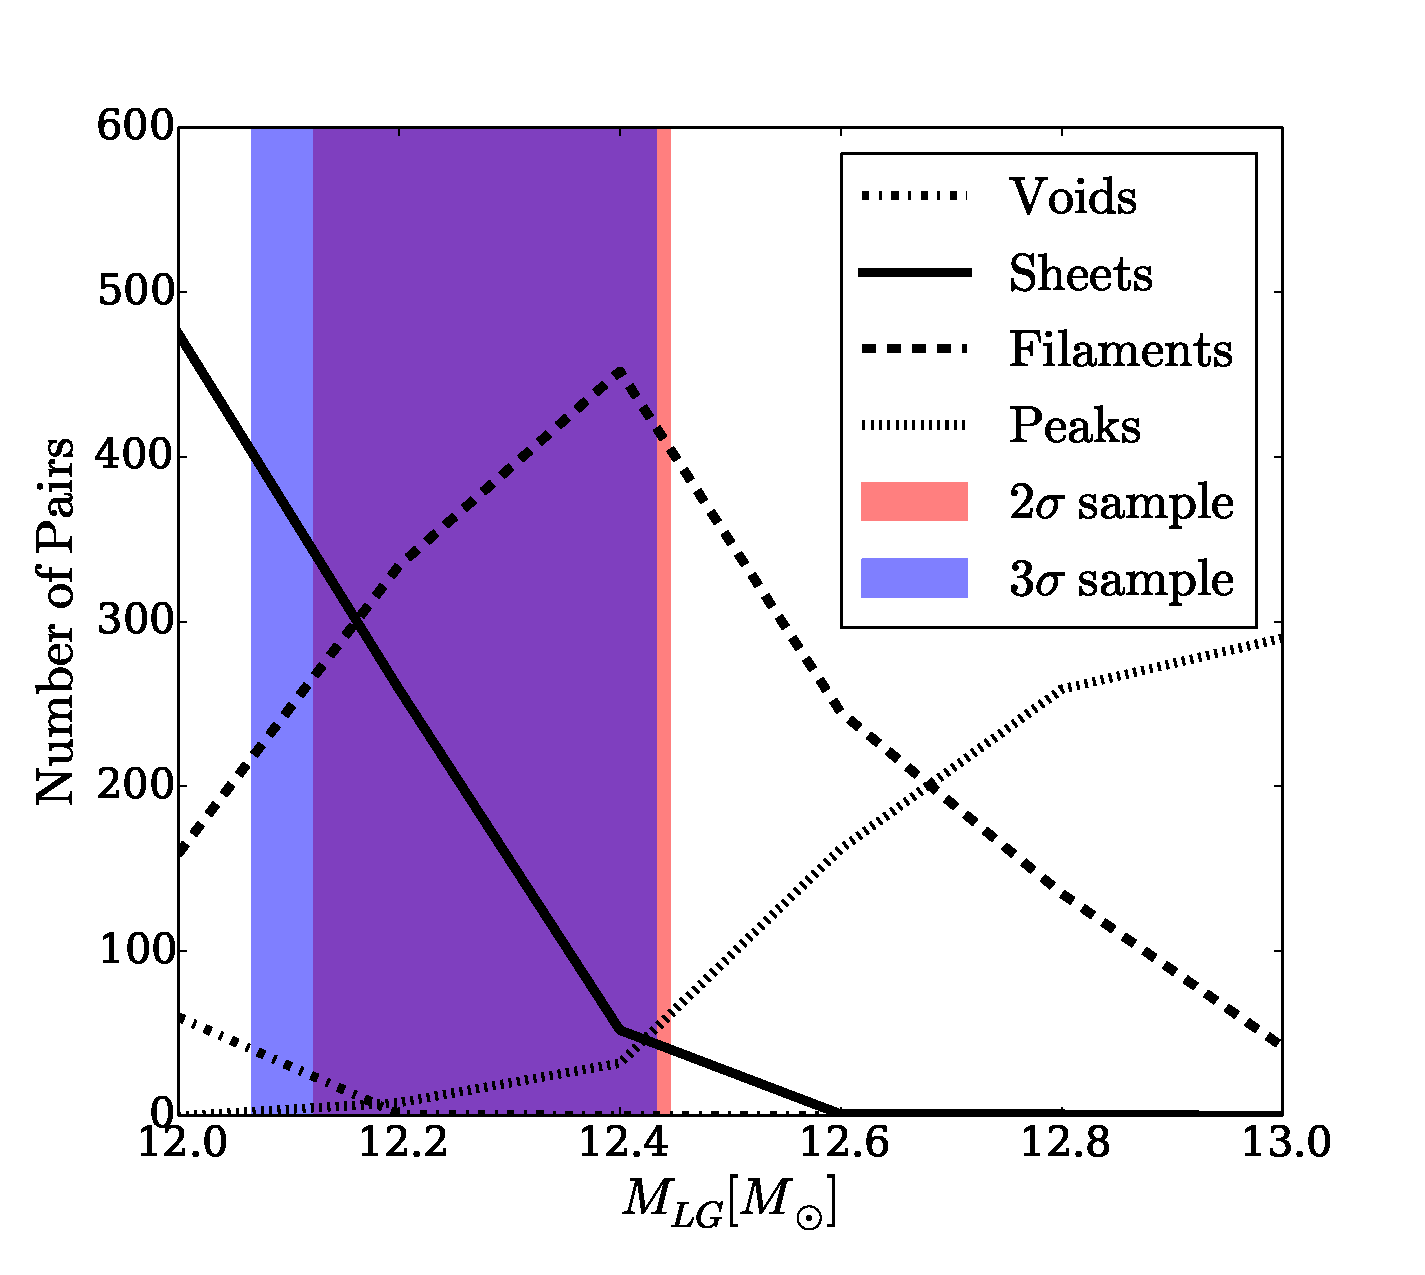
\includegraphics[width=0.48\textwidth]{histogram_mass_distro.pdf} 
%\caption{Mass dependency of the fraction of pairs in the different
%  environemnts.
%\label{fig:median_fraction}}
%\end{center}
%\end{figure}

\begin{figure}
\begin{center}
  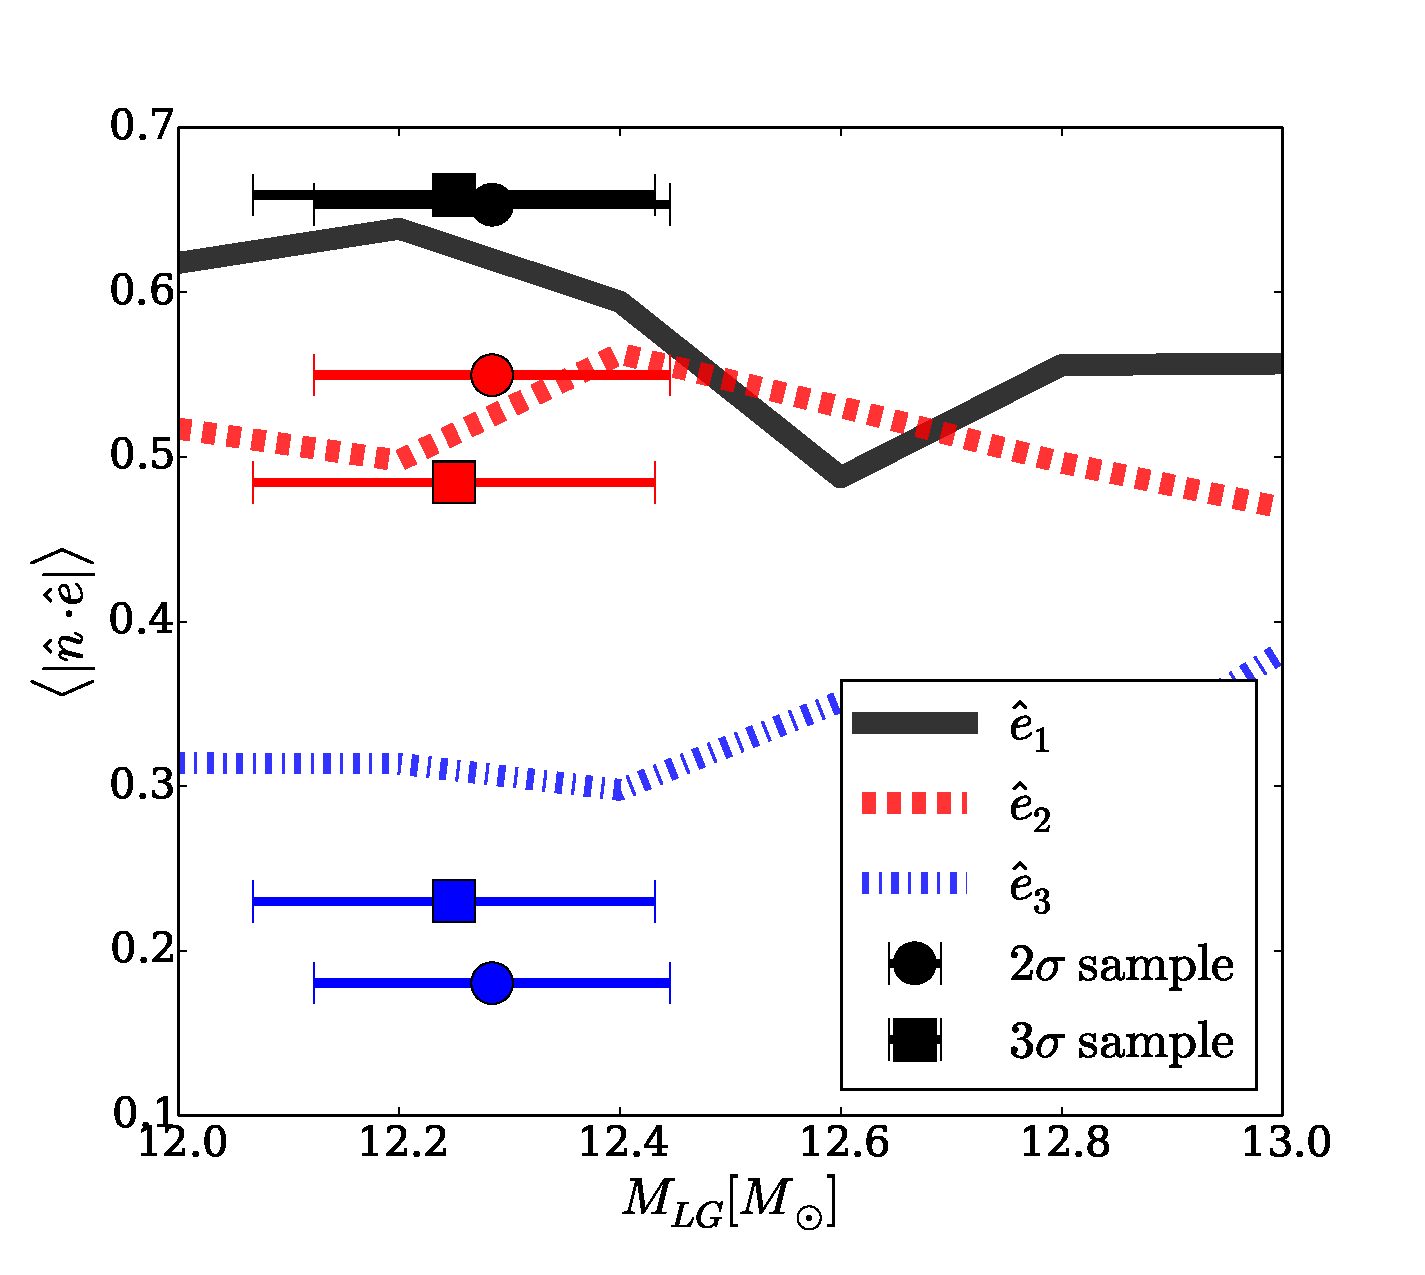
\includegraphics[width=0.48\textwidth]{median_mass_alignment.pdf}
\caption{Mass dependency of the median value for the dot product
  between the normal vector $\hat{n}$ and each one of the
  eigenvectors.  The lines show the trends for the general sample.
\label{fig:median_alignment_n}}
\end{center}
\end{figure}



\begin{figure}
\begin{center}
  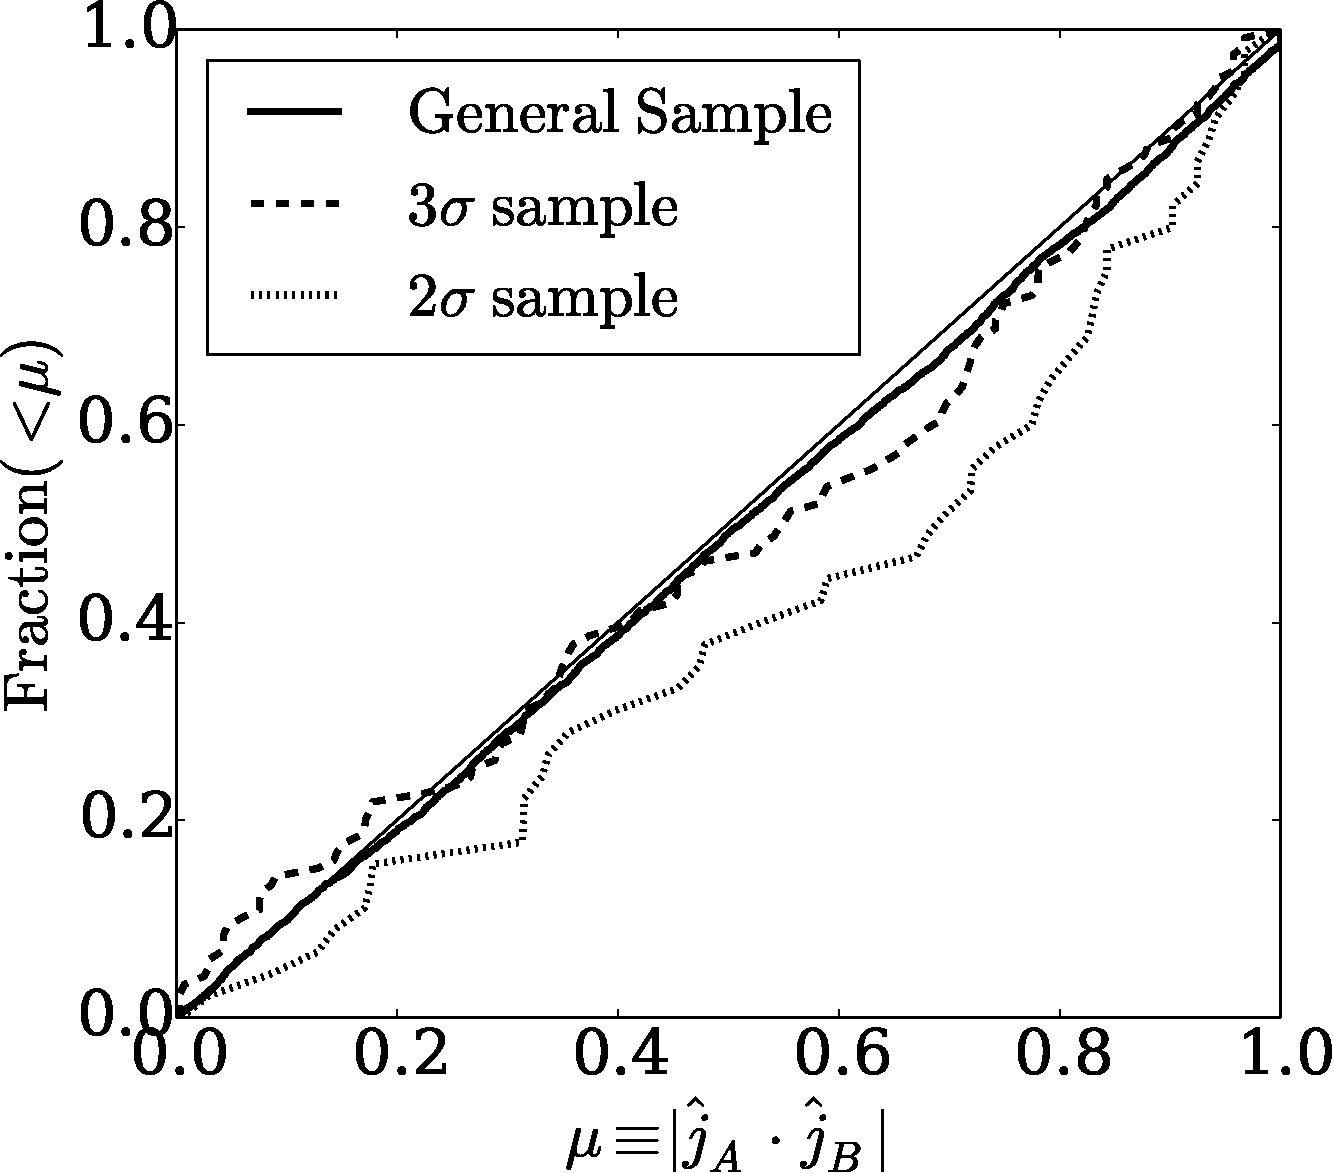
\includegraphics[width=0.49\textwidth]{alignments_jj_all_environments.pdf}
\end{center}
\caption{Alignment between the two angular momentum vectors of the two
  halos in the pair.
    \label{fig:jj_alignment}}  
\end{figure}



%\begin{figure*}
%\begin{center}
%  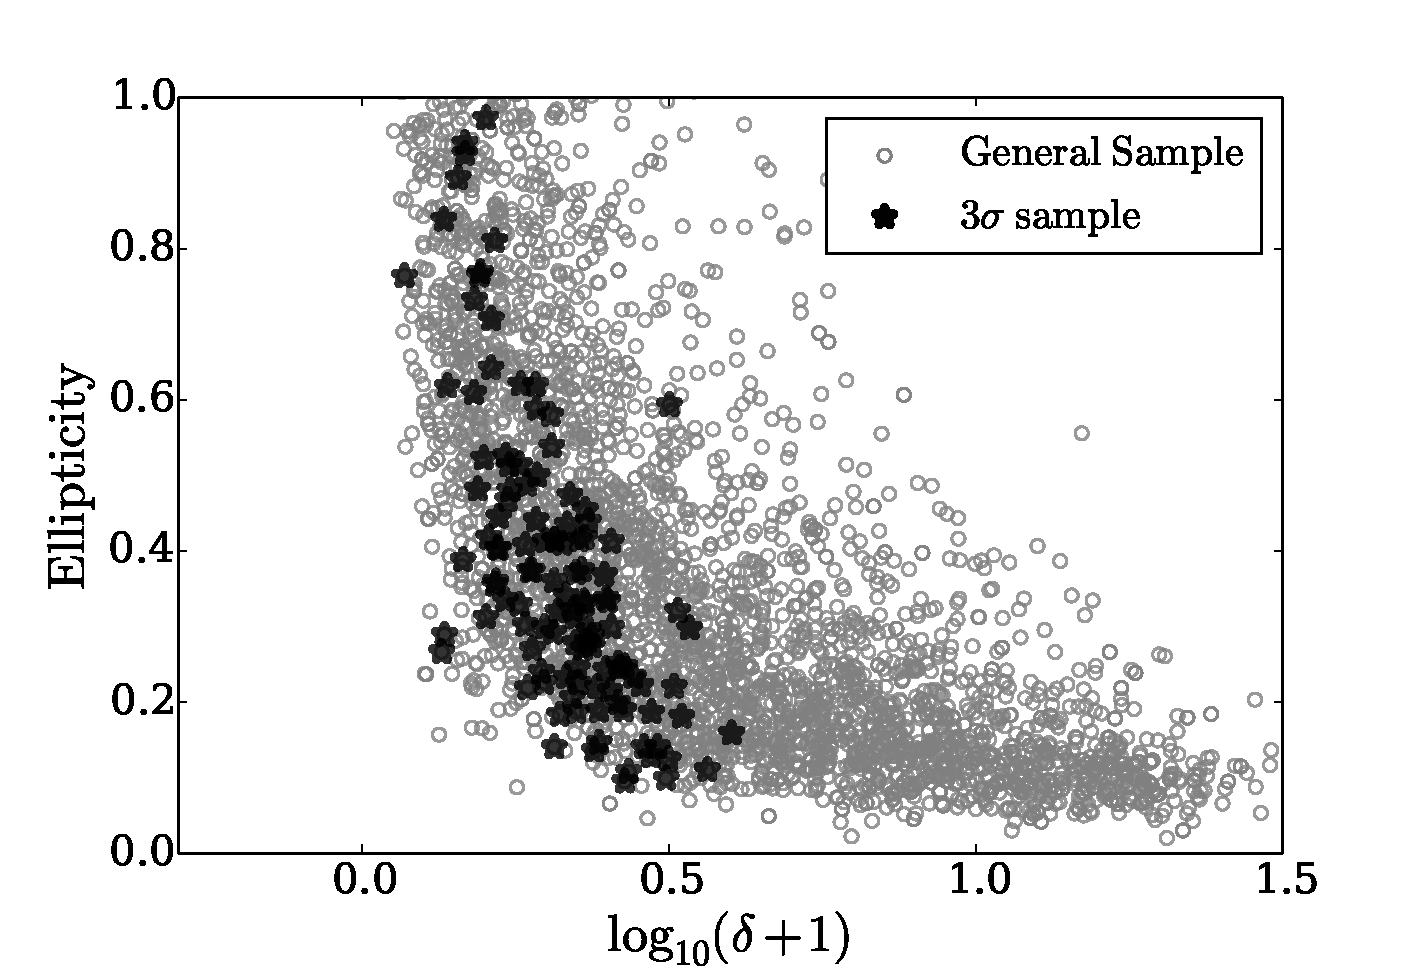
\includegraphics[width=0.49\textwidth]{ELL_delta_scatter.pdf}
%  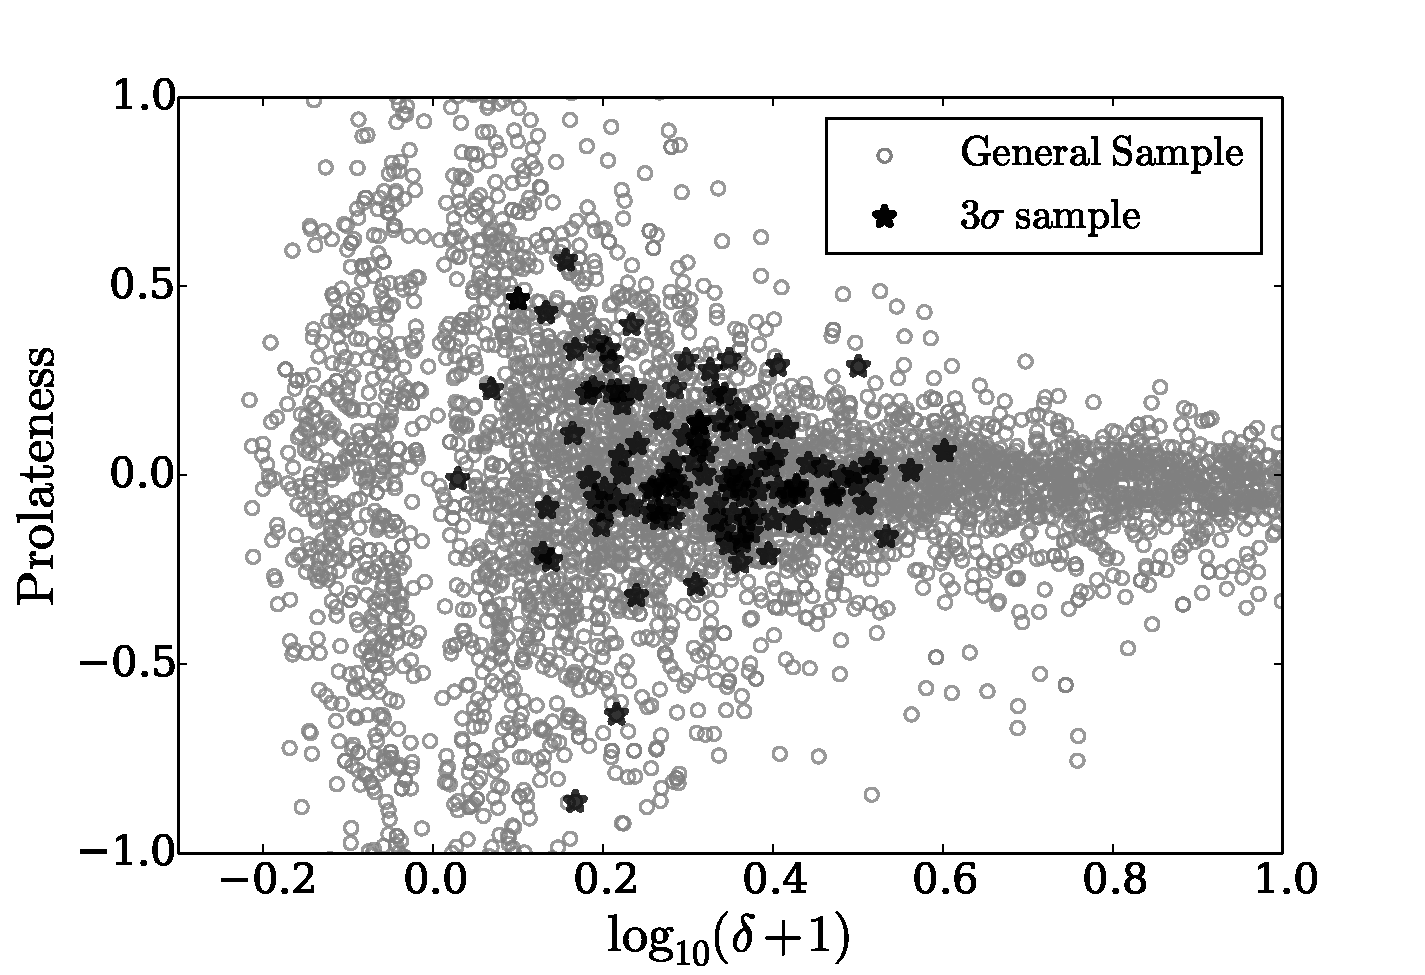
\includegraphics[width=0.49\textwidth]{PROL_delta_scatter.pdf}
%\end{center}
%\caption{Ellipticity and prolateness versus the overdensity for the pairs
%in the general and $3\sigma$ samples. \label{fig:delta_ELL_PROL}} 
%\end{figure*}


%\begin{figure}
%\begin{center}
%  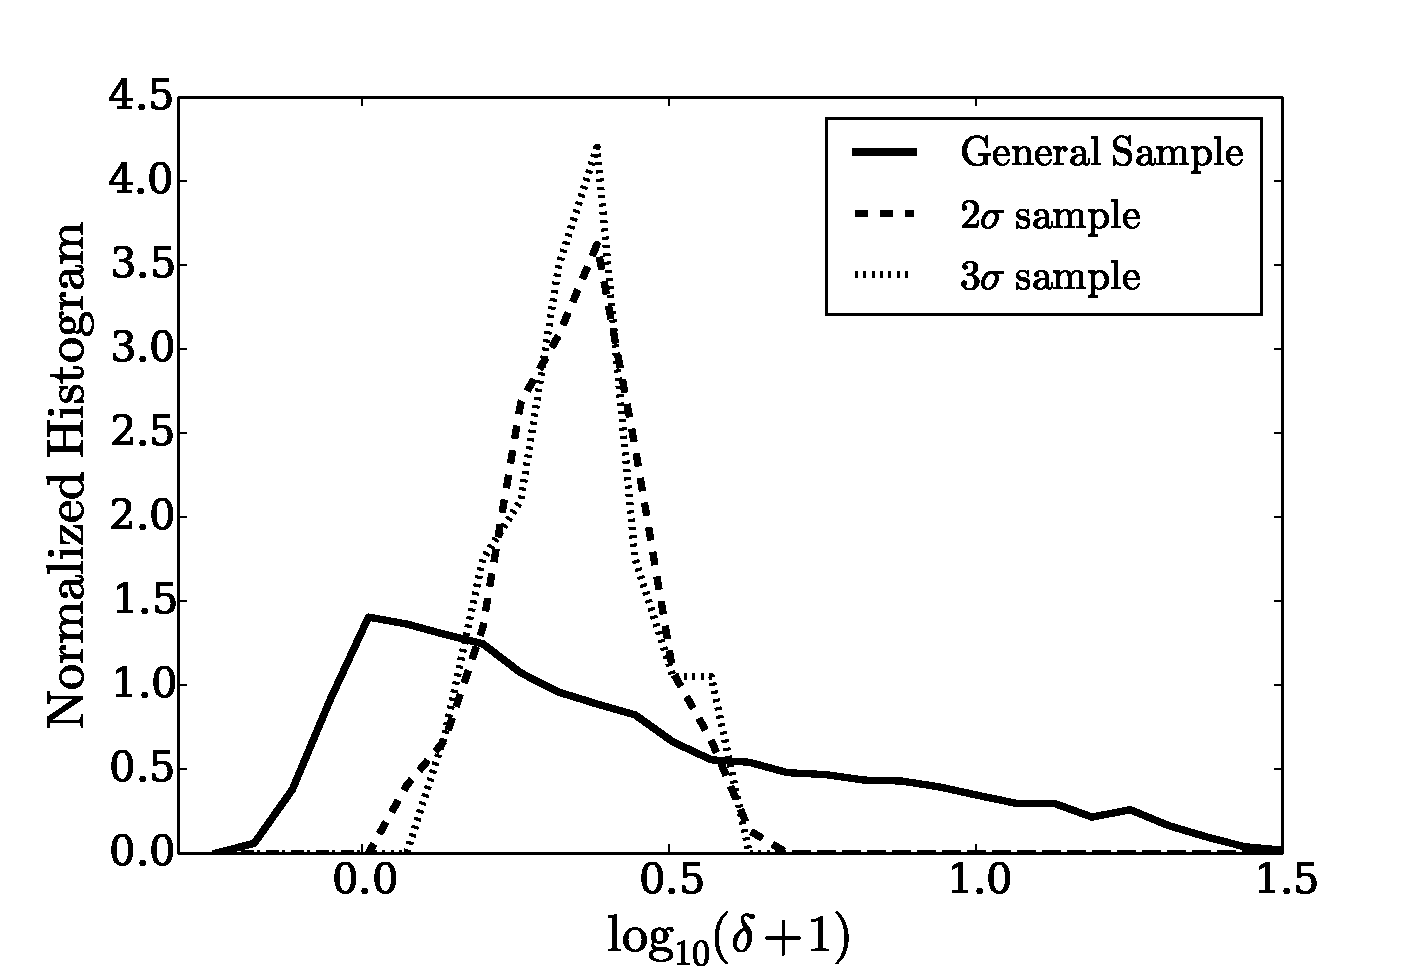
\includegraphics[width=0.50\textwidth]{density_histogram.pdf}
%\end{center}
%\caption{Overdensity distribution for the pairs in the three samples.
%    \label{fig:density}}  
%\end{figure}


\subsection{The prefered environment for LGs}

The first result we explore is the kind of environment occupied by
our LGs. 
We find that the LGs in the general sample are located across
all different evironment without any strong preferences; $1/3$  are
located in sheets, $1/4$ in peaks, $1/4$ in filaments and the remaning
$1/6$ in voids. 

The situation in the restricted $2\sigma$ and $3\sigma$ samples is very
different. 
By large the LGs in these samples are located in filaments and sheets. 
In both samples, $\sim 50\%$ of the pairs can be found in filaments
while $\sim 40\%$ are in sheets. 
These absolute numbers in each environment for each sample are
presented in Table \ref{table:web_type}.  

This difference between the general and the restricted samples is
due the mass ranges covered by each sample. 
In \citet{lganalogues} the mass range covered by $2\sigma$ and $3\sigma$ 
is very narrow and it is used to constraint the LG mass.
We show  in table \ref{table:web_type} that subset of the GS
having a similar mass range to $2\sigma$ and $3\sigma$ reproduces  
similar environment fractions.

Figure \ref{fig:median_fraction} clearly shows the correlation between
environment an total pair mass.
Each line represents the mass distribution of pairs in the four
different environments for the general sample.
High mass pairs tend to be located in  peaks and filaments while less
massive ones in voids and sheets. 
The shaded regions represent the $68\%$ confidence intervals of the mass 
distributions of $2\sigma$ and $3\sigma$ samples.



\subsection{Web Overdensity, Ellipticity and Anisotropy}

We now describe the preferred place of the LG samples in terms of the
web overdensity, ellipticiy and anisotropy as defined in Section
\ref{sec:simulation}. 

Figure \ref{fig:median_overdensity} shows dependency of the web overdensity,
ellipciticy, and prolateness on pair mass for the different samples.
GS is represented by the solid lines with the associated 
errors covered by the shaded region. 
The symbols represents the results for the $2\sigma$ and $3\sigma$
samples.  
In all cases it is immediatly clear that the range of values for the
$2\sigma$ and $3\sigma$ samples are completely expected from its mass
dependence.  

Left panel shows the overdensity dependence on pair mass. 
Higher mass pairs are located in high density regions.
The $2\sigma$ and $3\sigma$ samples having a narrower mass range as 
shown in previous figure, are consequently located within a narrower 
range of overdensities $0.0<\delta<4.0$ peaking at $\delta \sim 1$. 
This is also consistent with the fact that these samples are mostly 
found in filaments and sheets. 
The average overdensity of $2\sigma$ and $3\sigma$ samples is expected
from the values in the GS within the same mass range.

Middle and right panels show web ellipciticy and absolute prolateness
dependence on mass. Again we noticed that within the same mass range,
the $2\sigma$ and $3\sigma$ average ellipciticy and prolateness does not
differ significantly from GS
For the $2\sigma$ and $3\sigma$ samples most of the pairs are located
in a narrow range for ellipticities in the range $0.1<e<1.0$, and
prolateness $0.5<p<0.5$.

%the cumulative distribution for
%the ellipticity and prolateness. The general sample presents a wide
%range in ellipticity that can range from $-30<e<30$. For the $2\sigma$
%and $3\sigma$ samples most of the pairs are now located in a narrow
%range for ellipticities in the range $0.1<e<1.0$. This condition on
%the ellipticity together with the fact that $\delta>0$ implies that
%the prolateness in these samples must be bounded by
%$-1.0<p<1.0$. We actually find that they most of the pairs are bounded
%to an even narrower range $0.5<p<0.5$. 

%Figure \ref{fig:delta_FA} shows two panels with the joint scatter plot
%for the ellipticity and the prolateness as a function of the
%overdensity. For clarity we only include the general and $3\sigma$
%samples. In the left panel (ellipticity) we see the a simple cut in
%the overdensity is not enough to explain the narrow ranges in the
%ellipticity; the LG pairs in the $3\sigma$ sample are located towards
%low ellipticity values. In the right panel (prolateness) we find a
%similar situation; a cut in the overdensity would produced a wider
%distribution in prolateness values than the one featured by the
%$3\sigma$ sample.


\subsection{Alignment along the cosmic web}

We explore the alignment of the pairs with respect to the cosmic
web. 
We define the unit vector $\hat{n}$, normal to the pair orbital plane 
computed from the pair positions and relative velocity.
%First we define the unit vector $\hat{r}$ that links the two
%halos. 
Then, we compute the dot product of $\hat{n}$ and each one of
the three eigenvectors for the three samples. 

In Figure
\ref{fig:alignment} we show the main result of that study, it
presents the cumulative distribution of
$\mu\equiv\hat{e}_i\cdot\hat{n}$ for the three eigenvectors $i=1,2,3$. 
Lines indicate the different samples.
The straight line corresponds to the expected result for a
random vector distribution. 

From this Figure we can see two important features:
First, there is a strong anti-alignment signature between $\hat{n}$ 
and the third eigenvector, and this signature reverses with the first eigenvector.
However, in the case of the second eigenvector, no significant deviations are found.
Second, for $\hat{e}_3$ vector the anti-alignment become stronger for 
the samples more closely related to the LG, then for 2$\sigma$ it is 
stronger than for 3$\sigma$, and the latter is stronger than for General 
sample. 

%Figure \ref{fig:scheme} depicts a scheme of the alignment tendencies
%for pairs in all samples, where the pair members positions and 
%velocities tend to align with $\hat{e}_3$ vector.
%The alignment between the peculiar velocities and the $\hat{e}_3$ 
%eigenvector was already reported in \citet{ForeroRomero2014} for all
% halos regardles of its mass.

Quantitatively, the anti-alignment feature found with the $\hat{e}_3$ 
vector means that for 2$\sigma$ sample, $\sim 50\%$ pairs have $\mu<0.2$,
and $\sim 75\%$ pairs have $\mu<0.4$.
We also test that does not change significantly on environment type, in particular 
these trends hold very well for pairs in filaments and walls.

If we consider only pairs in filaments, we have that the pair orbit tends
to be perpendicular to the filament direction, and both pair members lie 
along the filament, if we recall the 3$\sigma$-2$\sigma$ samples are 
constrained with a mostly radial velocity component, then the pairs 
are moving into the filament.
In the case of sheets, we have the pair orbital plane  tend to lie within
 the sheet plane.

These alignment features are in agreement with the scenario that pairs 
created in-situ or falling into a filament/wall align their orbits with 
the large scale structure in a relaxation process where pair members
tend to moves along the slowest collapsing directions.
However, the most intriguing feature is the dependence of this alignment
with how close we represent the LG, is still not clear.
We explore if the pair masses are responsible of this, but we found 
no dependence at all.

In Figure \ref{fig:median_alignment_n} we show the relation between the median 
of $\mu\equiv\hat{e}_i\cdot\hat{n}$ and mass for the general sample, and found 
no significant relation.
Lines in the figure show the median $\mu$-mass relation for the three 
eigenvectors in the General sample.
Dots represent the median $\mu$ for the three eigenvectors in the 
2$\sigma$-3$\sigma$ samples.
In the case of $\|\hat{e}_3\cdot\hat{n}\|$, the figure clearly shows for a fixed mass
range around $1.5-2.0 \times 10^{10}$ \msun, that the median $\mu$ decreases as we
better constraint the LG samples, being larger for General sample and smaller for 
2$\sigma$ sample accordingly.


%From this Figure we first see that there is a clear distinct behavior
%between the general samples and the 3$\sigma$-2$\sigma$ samples. The
%general sample tend to be aligned along the $\hat{e}_3$ vector, the
%3$\sigma$ sample does not show any strong alignment and the 2$\sigma$
%pairs tend to be perpendicular to the $\hat{e}_3$ vector and slightly
%parallel to $\hat{e}_1$. These trends hold in filaments and walls.

%Let's focus on filaments first. That result means that in the general
%sample the two halos tend to lie along the filament, while in the
%2$\sigma$-3$\sigma$ samples they are located perpendicular to the
%filament. If one considers that in these samples the motion is radial,
%that means that the pairs are moving into the filament.

%In the case of sheets, the pairs in the general sample tend to lie on
%the sheet plane along the direction of the slowest collapsing
%direction. In the 2$\sigma$ samples the pairs are not constrained to
%the plane anymore and are perpendiculat to the $\hat{e}_3$
%vector. Considering the preferential radial motion of these pairs,
%that mens that the pairs are moving into the pancake all over a plane that
%is itself perpendicular to the sheet. 



\subsection{Spin and Orbital Angular Momentum}

In $4.2$ we defined the unit vector $\hat{n}$, normal to the pair 
orbital plane which can be asociated with the orbital angular 
momentum direction $\hat{J}$.
There, we show several alignment features of the pair orbital
momentum with the environment.
In this subsection we explore the alignement of the individual spin
angular momentum of each pair member $\hat{j_A}$ and $\hat{j_B}$ with
each other and with the orbital angular momentum.

We show in figure \ref{fig:jj_alignment} the cumulative distribution of
dot product between the spin of both members in the pair.
We found a slight alignment of spin vectors for the $2\sigma$ sample.
However, we found no significant alignment between spin and orbital angular 
momentum for any sample.

In the LG, the angle between MW and M31 spin is $\sim60^{\circ}$ and the
angles between spins and orbital angular momentum are $\sim33^{\circ}$
and $\sim76^{\circ}$ for MW and M31 respectively \citep{2012ApJ...753....9V}.
Then the LG show no particular alignement aswell. 

\section{Discussion}
\label{sec:discussion}

We explored the characteristics of the LG location in the cosmic web.

LG pairs are preferentially located in filaments and sheets. The mass range
of the pairs sample plays an important role in the fractions for each environment
type as shown in table $1$ and figure $1$.

There is a clear anti-alignment between the third eigenvector and the vector normal 
to the pair orbital plane. This feature is not mass dependant as can be shown in
figure $3$.
For pairs in filaments this means the pair orbit tends to be perpendicular to the 
filament direction, and both pair members lie along the filament, and in the case 
of pairs in sheets, we have the pair orbital plane lie in the sheet plane.
We also found this anti-alignment becomes stronger for the samples being more 
closely related to the LG, it means it is stronger for $2\sigma$ sample.
All these alignment features are consistent with pair orbits relaxing their 
movements towards the slowest collapsing directions at larger scales.

LG pairs are located in a narrow range of local overdensity, ellipciticy and prolateness.
And this is consistent with the narrow mass range selection of specific samples.

The LG spin and orbital angular momentum have no particular alignment,
and we see no significan alignments in our LG pairs, however for the alignment
between pair spins we found a slight alignment signature for $2\sigma$ sample as
can be seen in figure $5$.

\section{Conclusions}
\label{sec:conclusions}


\section*{Acknowledgements}
REG was supported by Proyecto Financiamiento Basal PFB06 and Comite Mixto ESO.

\bibliographystyle{apj}
\bibliography{references} 


\end{document}
